\documentclass[11pt, twoside]{article}
	\date{\LaTeX, Puteaux, 2020, 2021}
	\usepackage{fancyhdr}
	\usepackage{lastpage}
	\let\titleoriginal\title
	\renewcommand{\title}[1]{
		\titleoriginal{#1}
		\newcommand{\thetitle}{#1}}
	\fancypagestyle{plain}{
		\fancyhf{}
		\renewcommand{\headrulewidth}{0pt}
		\fancyfootoffset[RE]{-0.25\textwidth}
		\fancyfoot[R]{Page \thepage\ of \pageref{LastPage}}}
	\pagestyle{fancy}
	\fancyhf{}
	\renewcommand{\footrulewidth}{0.5pt}
	\fancyheadoffset[RE, LO]{-0.25\textwidth}
	\fancyfootoffset[RE, LO]{-0.25\textwidth}
	\fancyhead[LE,RO]{\thetitle}
	\fancyfoot[LE,RO]{Page \thepage\ of \pageref{LastPage}}
	\usepackage{wallpaper}
	\CenterWallPaper{}{../Figures/0. Wallpaper.jpg}

    \usepackage[breakable]{tcolorbox}
    \usepackage{parskip} % Stop auto-indenting (to mimic markdown behaviour)
    
    \usepackage{iftex}
    \ifPDFTeX
    	\usepackage[T1]{fontenc}
    	\usepackage{mathpazo}
    \else
    	\usepackage{fontspec}
    \fi

    % Basic figure setup, for now with no caption control since it's done
    % automatically by Pandoc (which extracts ![](path) syntax from Markdown).
    \usepackage{graphicx}
    % Maintain compatibility with old templates. Remove in nbconvert 6.0
    \let\Oldincludegraphics\includegraphics
    % Ensure that by default, figures have no caption (until we provide a
    % proper Figure object with a Caption API and a way to capture that
    % in the conversion process - todo).
    \usepackage{caption}
    \DeclareCaptionFormat{nocaption}{}
    \captionsetup{format=nocaption,aboveskip=0pt,belowskip=0pt}

    \usepackage[Export]{adjustbox} % Used to constrain images to a maximum size
    \adjustboxset{max size={0.9\linewidth}{0.9\paperheight}}
    \usepackage{float}
    \floatplacement{figure}{H} % forces figures to be placed at the correct location
    \usepackage{xcolor} % Allow colors to be defined
    \usepackage{enumerate} % Needed for markdown enumerations to work
    \usepackage{geometry} % Used to adjust the document margins
    \usepackage{amsmath} % Equations
    \usepackage{amssymb} % Equations
    \usepackage{textcomp} % defines textquotesingle
    % Hack from http://tex.stackexchange.com/a/47451/13684:
    \AtBeginDocument{%
        \def\PYZsq{\textquotesingle}% Upright quotes in Pygmentized code
    }
    \usepackage{upquote} % Upright quotes for verbatim code
    \usepackage{eurosym} % defines \euro
    \usepackage[mathletters]{ucs} % Extended unicode (utf-8) support
    \usepackage{fancyvrb} % verbatim replacement that allows latex
    \usepackage{grffile} % extends the file name processing of package graphics 
                         % to support a larger range
    \makeatletter % fix for grffile with XeLaTeX
    \def\Gread@@xetex#1{%
      \IfFileExists{"\Gin@base".bb}%
      {\Gread@eps{\Gin@base.bb}}%
      {\Gread@@xetex@aux#1}%
    }
    \makeatother

    % The hyperref package gives us a pdf with properly built
    % internal navigation ('pdf bookmarks' for the table of contents,
    % internal cross-reference links, web links for URLs, etc.)
    \usepackage{hyperref}
    % The default LaTeX title has an obnoxious amount of whitespace. By default,
    % titling removes some of it. It also provides customization options.
    \usepackage{titling}
    \usepackage{longtable} % longtable support required by pandoc >1.10
    \usepackage{booktabs}  % table support for pandoc > 1.12.2
    \usepackage[inline]{enumitem} % IRkernel/repr support (it uses the enumerate* environment)
    \usepackage[normalem]{ulem} % ulem is needed to support strikethroughs (\sout)
                                % normalem makes italics be italics, not underlines
    \usepackage{mathrsfs}
    

    
    % Colors for the hyperref package
    \definecolor{urlcolor}{rgb}{0,.145,.698}
    \definecolor{linkcolor}{rgb}{.71,0.21,0.01}
    \definecolor{citecolor}{rgb}{.12,.54,.11}

    % ANSI colors
    \definecolor{ansi-black}{HTML}{3E424D}
    \definecolor{ansi-black-intense}{HTML}{282C36}
    \definecolor{ansi-red}{HTML}{E75C58}
    \definecolor{ansi-red-intense}{HTML}{B22B31}
    \definecolor{ansi-green}{HTML}{00A250}
    \definecolor{ansi-green-intense}{HTML}{007427}
    \definecolor{ansi-yellow}{HTML}{DDB62B}
    \definecolor{ansi-yellow-intense}{HTML}{B27D12}
    \definecolor{ansi-blue}{HTML}{208FFB}
    \definecolor{ansi-blue-intense}{HTML}{0065CA}
    \definecolor{ansi-magenta}{HTML}{D160C4}
    \definecolor{ansi-magenta-intense}{HTML}{A03196}
    \definecolor{ansi-cyan}{HTML}{60C6C8}
    \definecolor{ansi-cyan-intense}{HTML}{258F8F}
    \definecolor{ansi-white}{HTML}{C5C1B4}
    \definecolor{ansi-white-intense}{HTML}{A1A6B2}
    \definecolor{ansi-default-inverse-fg}{HTML}{FFFFFF}
    \definecolor{ansi-default-inverse-bg}{HTML}{000000}

    % commands and environments needed by pandoc snippets
    % extracted from the output of `pandoc -s`
    \providecommand{\tightlist}{%
      \setlength{\itemsep}{0pt}\setlength{\parskip}{0pt}}
    \DefineVerbatimEnvironment{Highlighting}{Verbatim}{commandchars=\\\{\}}
    % Add ',fontsize=\small' for more characters per line
    \newenvironment{Shaded}{}{}
    \newcommand{\KeywordTok}[1]{\textcolor[rgb]{0.00,0.44,0.13}{\textbf{{#1}}}}
    \newcommand{\DataTypeTok}[1]{\textcolor[rgb]{0.56,0.13,0.00}{{#1}}}
    \newcommand{\DecValTok}[1]{\textcolor[rgb]{0.25,0.63,0.44}{{#1}}}
    \newcommand{\BaseNTok}[1]{\textcolor[rgb]{0.25,0.63,0.44}{{#1}}}
    \newcommand{\FloatTok}[1]{\textcolor[rgb]{0.25,0.63,0.44}{{#1}}}
    \newcommand{\CharTok}[1]{\textcolor[rgb]{0.25,0.44,0.63}{{#1}}}
    \newcommand{\StringTok}[1]{\textcolor[rgb]{0.25,0.44,0.63}{{#1}}}
    \newcommand{\CommentTok}[1]{\textcolor[rgb]{0.38,0.63,0.69}{\textit{{#1}}}}
    \newcommand{\OtherTok}[1]{\textcolor[rgb]{0.00,0.44,0.13}{{#1}}}
    \newcommand{\AlertTok}[1]{\textcolor[rgb]{1.00,0.00,0.00}{\textbf{{#1}}}}
    \newcommand{\FunctionTok}[1]{\textcolor[rgb]{0.02,0.16,0.49}{{#1}}}
    \newcommand{\RegionMarkerTok}[1]{{#1}}
    \newcommand{\ErrorTok}[1]{\textcolor[rgb]{1.00,0.00,0.00}{\textbf{{#1}}}}
    \newcommand{\NormalTok}[1]{{#1}}
    
    % Additional commands for more recent versions of Pandoc
    \newcommand{\ConstantTok}[1]{\textcolor[rgb]{0.53,0.00,0.00}{{#1}}}
    \newcommand{\SpecialCharTok}[1]{\textcolor[rgb]{0.25,0.44,0.63}{{#1}}}
    \newcommand{\VerbatimStringTok}[1]{\textcolor[rgb]{0.25,0.44,0.63}{{#1}}}
    \newcommand{\SpecialStringTok}[1]{\textcolor[rgb]{0.73,0.40,0.53}{{#1}}}
    \newcommand{\ImportTok}[1]{{#1}}
    \newcommand{\DocumentationTok}[1]{\textcolor[rgb]{0.73,0.13,0.13}{\textit{{#1}}}}
    \newcommand{\AnnotationTok}[1]{\textcolor[rgb]{0.38,0.63,0.69}{\textbf{\textit{{#1}}}}}
    \newcommand{\CommentVarTok}[1]{\textcolor[rgb]{0.38,0.63,0.69}{\textbf{\textit{{#1}}}}}
    \newcommand{\VariableTok}[1]{\textcolor[rgb]{0.10,0.09,0.49}{{#1}}}
    \newcommand{\ControlFlowTok}[1]{\textcolor[rgb]{0.00,0.44,0.13}{\textbf{{#1}}}}
    \newcommand{\OperatorTok}[1]{\textcolor[rgb]{0.40,0.40,0.40}{{#1}}}
    \newcommand{\BuiltInTok}[1]{{#1}}
    \newcommand{\ExtensionTok}[1]{{#1}}
    \newcommand{\PreprocessorTok}[1]{\textcolor[rgb]{0.74,0.48,0.00}{{#1}}}
    \newcommand{\AttributeTok}[1]{\textcolor[rgb]{0.49,0.56,0.16}{{#1}}}
    \newcommand{\InformationTok}[1]{\textcolor[rgb]{0.38,0.63,0.69}{\textbf{\textit{{#1}}}}}
    \newcommand{\WarningTok}[1]{\textcolor[rgb]{0.38,0.63,0.69}{\textbf{\textit{{#1}}}}}
    
    
    % Define a nice break command that doesn't care if a line doesn't already
    % exist.
    \def\br{\hspace*{\fill} \\* }
    % Math Jax compatibility definitions
    \def\gt{>}
    \def\lt{<}
    \let\Oldtex\TeX
    \let\Oldlatex\LaTeX
    \renewcommand{\TeX}{\textrm{\Oldtex}}
    \renewcommand{\LaTeX}{\textrm{\Oldlatex}}
    % Document parameters
    % Document title
    \title{Basics of Deep Learning and Neural Networks}
    
    
    
    
    
% Pygments definitions
\makeatletter
\def\PY@reset{\let\PY@it=\relax \let\PY@bf=\relax%
    \let\PY@ul=\relax \let\PY@tc=\relax%
    \let\PY@bc=\relax \let\PY@ff=\relax}
\def\PY@tok#1{\csname PY@tok@#1\endcsname}
\def\PY@toks#1+{\ifx\relax#1\empty\else%
    \PY@tok{#1}\expandafter\PY@toks\fi}
\def\PY@do#1{\PY@bc{\PY@tc{\PY@ul{%
    \PY@it{\PY@bf{\PY@ff{#1}}}}}}}
\def\PY#1#2{\PY@reset\PY@toks#1+\relax+\PY@do{#2}}

\expandafter\def\csname PY@tok@w\endcsname{\def\PY@tc##1{\textcolor[rgb]{0.73,0.73,0.73}{##1}}}
\expandafter\def\csname PY@tok@c\endcsname{\let\PY@it=\textit\def\PY@tc##1{\textcolor[rgb]{0.25,0.50,0.50}{##1}}}
\expandafter\def\csname PY@tok@cp\endcsname{\def\PY@tc##1{\textcolor[rgb]{0.74,0.48,0.00}{##1}}}
\expandafter\def\csname PY@tok@k\endcsname{\let\PY@bf=\textbf\def\PY@tc##1{\textcolor[rgb]{0.00,0.50,0.00}{##1}}}
\expandafter\def\csname PY@tok@kp\endcsname{\def\PY@tc##1{\textcolor[rgb]{0.00,0.50,0.00}{##1}}}
\expandafter\def\csname PY@tok@kt\endcsname{\def\PY@tc##1{\textcolor[rgb]{0.69,0.00,0.25}{##1}}}
\expandafter\def\csname PY@tok@o\endcsname{\def\PY@tc##1{\textcolor[rgb]{0.40,0.40,0.40}{##1}}}
\expandafter\def\csname PY@tok@ow\endcsname{\let\PY@bf=\textbf\def\PY@tc##1{\textcolor[rgb]{0.67,0.13,1.00}{##1}}}
\expandafter\def\csname PY@tok@nb\endcsname{\def\PY@tc##1{\textcolor[rgb]{0.00,0.50,0.00}{##1}}}
\expandafter\def\csname PY@tok@nf\endcsname{\def\PY@tc##1{\textcolor[rgb]{0.00,0.00,1.00}{##1}}}
\expandafter\def\csname PY@tok@nc\endcsname{\let\PY@bf=\textbf\def\PY@tc##1{\textcolor[rgb]{0.00,0.00,1.00}{##1}}}
\expandafter\def\csname PY@tok@nn\endcsname{\let\PY@bf=\textbf\def\PY@tc##1{\textcolor[rgb]{0.00,0.00,1.00}{##1}}}
\expandafter\def\csname PY@tok@ne\endcsname{\let\PY@bf=\textbf\def\PY@tc##1{\textcolor[rgb]{0.82,0.25,0.23}{##1}}}
\expandafter\def\csname PY@tok@nv\endcsname{\def\PY@tc##1{\textcolor[rgb]{0.10,0.09,0.49}{##1}}}
\expandafter\def\csname PY@tok@no\endcsname{\def\PY@tc##1{\textcolor[rgb]{0.53,0.00,0.00}{##1}}}
\expandafter\def\csname PY@tok@nl\endcsname{\def\PY@tc##1{\textcolor[rgb]{0.63,0.63,0.00}{##1}}}
\expandafter\def\csname PY@tok@ni\endcsname{\let\PY@bf=\textbf\def\PY@tc##1{\textcolor[rgb]{0.60,0.60,0.60}{##1}}}
\expandafter\def\csname PY@tok@na\endcsname{\def\PY@tc##1{\textcolor[rgb]{0.49,0.56,0.16}{##1}}}
\expandafter\def\csname PY@tok@nt\endcsname{\let\PY@bf=\textbf\def\PY@tc##1{\textcolor[rgb]{0.00,0.50,0.00}{##1}}}
\expandafter\def\csname PY@tok@nd\endcsname{\def\PY@tc##1{\textcolor[rgb]{0.67,0.13,1.00}{##1}}}
\expandafter\def\csname PY@tok@s\endcsname{\def\PY@tc##1{\textcolor[rgb]{0.73,0.13,0.13}{##1}}}
\expandafter\def\csname PY@tok@sd\endcsname{\let\PY@it=\textit\def\PY@tc##1{\textcolor[rgb]{0.73,0.13,0.13}{##1}}}
\expandafter\def\csname PY@tok@si\endcsname{\let\PY@bf=\textbf\def\PY@tc##1{\textcolor[rgb]{0.73,0.40,0.53}{##1}}}
\expandafter\def\csname PY@tok@se\endcsname{\let\PY@bf=\textbf\def\PY@tc##1{\textcolor[rgb]{0.73,0.40,0.13}{##1}}}
\expandafter\def\csname PY@tok@sr\endcsname{\def\PY@tc##1{\textcolor[rgb]{0.73,0.40,0.53}{##1}}}
\expandafter\def\csname PY@tok@ss\endcsname{\def\PY@tc##1{\textcolor[rgb]{0.10,0.09,0.49}{##1}}}
\expandafter\def\csname PY@tok@sx\endcsname{\def\PY@tc##1{\textcolor[rgb]{0.00,0.50,0.00}{##1}}}
\expandafter\def\csname PY@tok@m\endcsname{\def\PY@tc##1{\textcolor[rgb]{0.40,0.40,0.40}{##1}}}
\expandafter\def\csname PY@tok@gh\endcsname{\let\PY@bf=\textbf\def\PY@tc##1{\textcolor[rgb]{0.00,0.00,0.50}{##1}}}
\expandafter\def\csname PY@tok@gu\endcsname{\let\PY@bf=\textbf\def\PY@tc##1{\textcolor[rgb]{0.50,0.00,0.50}{##1}}}
\expandafter\def\csname PY@tok@gd\endcsname{\def\PY@tc##1{\textcolor[rgb]{0.63,0.00,0.00}{##1}}}
\expandafter\def\csname PY@tok@gi\endcsname{\def\PY@tc##1{\textcolor[rgb]{0.00,0.63,0.00}{##1}}}
\expandafter\def\csname PY@tok@gr\endcsname{\def\PY@tc##1{\textcolor[rgb]{1.00,0.00,0.00}{##1}}}
\expandafter\def\csname PY@tok@ge\endcsname{\let\PY@it=\textit}
\expandafter\def\csname PY@tok@gs\endcsname{\let\PY@bf=\textbf}
\expandafter\def\csname PY@tok@gp\endcsname{\let\PY@bf=\textbf\def\PY@tc##1{\textcolor[rgb]{0.00,0.00,0.50}{##1}}}
\expandafter\def\csname PY@tok@go\endcsname{\def\PY@tc##1{\textcolor[rgb]{0.53,0.53,0.53}{##1}}}
\expandafter\def\csname PY@tok@gt\endcsname{\def\PY@tc##1{\textcolor[rgb]{0.00,0.27,0.87}{##1}}}
\expandafter\def\csname PY@tok@err\endcsname{\def\PY@bc##1{\setlength{\fboxsep}{0pt}\fcolorbox[rgb]{1.00,0.00,0.00}{1,1,1}{\strut ##1}}}
\expandafter\def\csname PY@tok@kc\endcsname{\let\PY@bf=\textbf\def\PY@tc##1{\textcolor[rgb]{0.00,0.50,0.00}{##1}}}
\expandafter\def\csname PY@tok@kd\endcsname{\let\PY@bf=\textbf\def\PY@tc##1{\textcolor[rgb]{0.00,0.50,0.00}{##1}}}
\expandafter\def\csname PY@tok@kn\endcsname{\let\PY@bf=\textbf\def\PY@tc##1{\textcolor[rgb]{0.00,0.50,0.00}{##1}}}
\expandafter\def\csname PY@tok@kr\endcsname{\let\PY@bf=\textbf\def\PY@tc##1{\textcolor[rgb]{0.00,0.50,0.00}{##1}}}
\expandafter\def\csname PY@tok@bp\endcsname{\def\PY@tc##1{\textcolor[rgb]{0.00,0.50,0.00}{##1}}}
\expandafter\def\csname PY@tok@fm\endcsname{\def\PY@tc##1{\textcolor[rgb]{0.00,0.00,1.00}{##1}}}
\expandafter\def\csname PY@tok@vc\endcsname{\def\PY@tc##1{\textcolor[rgb]{0.10,0.09,0.49}{##1}}}
\expandafter\def\csname PY@tok@vg\endcsname{\def\PY@tc##1{\textcolor[rgb]{0.10,0.09,0.49}{##1}}}
\expandafter\def\csname PY@tok@vi\endcsname{\def\PY@tc##1{\textcolor[rgb]{0.10,0.09,0.49}{##1}}}
\expandafter\def\csname PY@tok@vm\endcsname{\def\PY@tc##1{\textcolor[rgb]{0.10,0.09,0.49}{##1}}}
\expandafter\def\csname PY@tok@sa\endcsname{\def\PY@tc##1{\textcolor[rgb]{0.73,0.13,0.13}{##1}}}
\expandafter\def\csname PY@tok@sb\endcsname{\def\PY@tc##1{\textcolor[rgb]{0.73,0.13,0.13}{##1}}}
\expandafter\def\csname PY@tok@sc\endcsname{\def\PY@tc##1{\textcolor[rgb]{0.73,0.13,0.13}{##1}}}
\expandafter\def\csname PY@tok@dl\endcsname{\def\PY@tc##1{\textcolor[rgb]{0.73,0.13,0.13}{##1}}}
\expandafter\def\csname PY@tok@s2\endcsname{\def\PY@tc##1{\textcolor[rgb]{0.73,0.13,0.13}{##1}}}
\expandafter\def\csname PY@tok@sh\endcsname{\def\PY@tc##1{\textcolor[rgb]{0.73,0.13,0.13}{##1}}}
\expandafter\def\csname PY@tok@s1\endcsname{\def\PY@tc##1{\textcolor[rgb]{0.73,0.13,0.13}{##1}}}
\expandafter\def\csname PY@tok@mb\endcsname{\def\PY@tc##1{\textcolor[rgb]{0.40,0.40,0.40}{##1}}}
\expandafter\def\csname PY@tok@mf\endcsname{\def\PY@tc##1{\textcolor[rgb]{0.40,0.40,0.40}{##1}}}
\expandafter\def\csname PY@tok@mh\endcsname{\def\PY@tc##1{\textcolor[rgb]{0.40,0.40,0.40}{##1}}}
\expandafter\def\csname PY@tok@mi\endcsname{\def\PY@tc##1{\textcolor[rgb]{0.40,0.40,0.40}{##1}}}
\expandafter\def\csname PY@tok@il\endcsname{\def\PY@tc##1{\textcolor[rgb]{0.40,0.40,0.40}{##1}}}
\expandafter\def\csname PY@tok@mo\endcsname{\def\PY@tc##1{\textcolor[rgb]{0.40,0.40,0.40}{##1}}}
\expandafter\def\csname PY@tok@ch\endcsname{\let\PY@it=\textit\def\PY@tc##1{\textcolor[rgb]{0.25,0.50,0.50}{##1}}}
\expandafter\def\csname PY@tok@cm\endcsname{\let\PY@it=\textit\def\PY@tc##1{\textcolor[rgb]{0.25,0.50,0.50}{##1}}}
\expandafter\def\csname PY@tok@cpf\endcsname{\let\PY@it=\textit\def\PY@tc##1{\textcolor[rgb]{0.25,0.50,0.50}{##1}}}
\expandafter\def\csname PY@tok@c1\endcsname{\let\PY@it=\textit\def\PY@tc##1{\textcolor[rgb]{0.25,0.50,0.50}{##1}}}
\expandafter\def\csname PY@tok@cs\endcsname{\let\PY@it=\textit\def\PY@tc##1{\textcolor[rgb]{0.25,0.50,0.50}{##1}}}

\def\PYZbs{\char`\\}
\def\PYZus{\char`\_}
\def\PYZob{\char`\{}
\def\PYZcb{\char`\}}
\def\PYZca{\char`\^}
\def\PYZam{\char`\&}
\def\PYZlt{\char`\<}
\def\PYZgt{\char`\>}
\def\PYZsh{\char`\#}
\def\PYZpc{\char`\%}
\def\PYZdl{\char`\$}
\def\PYZhy{\char`\-}
\def\PYZsq{\char`\'}
\def\PYZdq{\char`\"}
\def\PYZti{\char`\~}
% for compatibility with earlier versions
\def\PYZat{@}
\def\PYZlb{[}
\def\PYZrb{]}
\makeatother


    % For linebreaks inside Verbatim environment from package fancyvrb. 
    \makeatletter
        \newbox\Wrappedcontinuationbox 
        \newbox\Wrappedvisiblespacebox 
        \newcommand*\Wrappedvisiblespace {\textcolor{red}{\textvisiblespace}} 
        \newcommand*\Wrappedcontinuationsymbol {\textcolor{red}{\llap{\tiny$\m@th\hookrightarrow$}}} 
        \newcommand*\Wrappedcontinuationindent {3ex } 
        \newcommand*\Wrappedafterbreak {\kern\Wrappedcontinuationindent\copy\Wrappedcontinuationbox} 
        % Take advantage of the already applied Pygments mark-up to insert 
        % potential linebreaks for TeX processing. 
        %        {, <, #, %, $, ' and ": go to next line. 
        %        _, }, ^, &, >, - and ~: stay at end of broken line. 
        % Use of \textquotesingle for straight quote. 
        \newcommand*\Wrappedbreaksatspecials {% 
            \def\PYGZus{\discretionary{\char`\_}{\Wrappedafterbreak}{\char`\_}}% 
            \def\PYGZob{\discretionary{}{\Wrappedafterbreak\char`\{}{\char`\{}}% 
            \def\PYGZcb{\discretionary{\char`\}}{\Wrappedafterbreak}{\char`\}}}% 
            \def\PYGZca{\discretionary{\char`\^}{\Wrappedafterbreak}{\char`\^}}% 
            \def\PYGZam{\discretionary{\char`\&}{\Wrappedafterbreak}{\char`\&}}% 
            \def\PYGZlt{\discretionary{}{\Wrappedafterbreak\char`\<}{\char`\<}}% 
            \def\PYGZgt{\discretionary{\char`\>}{\Wrappedafterbreak}{\char`\>}}% 
            \def\PYGZsh{\discretionary{}{\Wrappedafterbreak\char`\#}{\char`\#}}% 
            \def\PYGZpc{\discretionary{}{\Wrappedafterbreak\char`\%}{\char`\%}}% 
            \def\PYGZdl{\discretionary{}{\Wrappedafterbreak\char`\$}{\char`\$}}% 
            \def\PYGZhy{\discretionary{\char`\-}{\Wrappedafterbreak}{\char`\-}}% 
            \def\PYGZsq{\discretionary{}{\Wrappedafterbreak\textquotesingle}{\textquotesingle}}% 
            \def\PYGZdq{\discretionary{}{\Wrappedafterbreak\char`\"}{\char`\"}}% 
            \def\PYGZti{\discretionary{\char`\~}{\Wrappedafterbreak}{\char`\~}}% 
        } 
        % Some characters . , ; ? ! / are not pygmentized. 
        % This macro makes them "active" and they will insert potential linebreaks 
        \newcommand*\Wrappedbreaksatpunct {% 
            \lccode`\~`\.\lowercase{\def~}{\discretionary{\hbox{\char`\.}}{\Wrappedafterbreak}{\hbox{\char`\.}}}% 
            \lccode`\~`\,\lowercase{\def~}{\discretionary{\hbox{\char`\,}}{\Wrappedafterbreak}{\hbox{\char`\,}}}% 
            \lccode`\~`\;\lowercase{\def~}{\discretionary{\hbox{\char`\;}}{\Wrappedafterbreak}{\hbox{\char`\;}}}% 
            \lccode`\~`\:\lowercase{\def~}{\discretionary{\hbox{\char`\:}}{\Wrappedafterbreak}{\hbox{\char`\:}}}% 
            \lccode`\~`\?\lowercase{\def~}{\discretionary{\hbox{\char`\?}}{\Wrappedafterbreak}{\hbox{\char`\?}}}% 
            \lccode`\~`\!\lowercase{\def~}{\discretionary{\hbox{\char`\!}}{\Wrappedafterbreak}{\hbox{\char`\!}}}% 
            \lccode`\~`\/\lowercase{\def~}{\discretionary{\hbox{\char`\/}}{\Wrappedafterbreak}{\hbox{\char`\/}}}% 
            \catcode`\.\active
            \catcode`\,\active 
            \catcode`\;\active
            \catcode`\:\active
            \catcode`\?\active
            \catcode`\!\active
            \catcode`\/\active 
            \lccode`\~`\~ 	
        }
    \makeatother

    \let\OriginalVerbatim=\Verbatim
    \makeatletter
    \renewcommand{\Verbatim}[1][1]{%
        %\parskip\z@skip
        \sbox\Wrappedcontinuationbox {\Wrappedcontinuationsymbol}%
        \sbox\Wrappedvisiblespacebox {\FV@SetupFont\Wrappedvisiblespace}%
        \def\FancyVerbFormatLine ##1{\hsize\linewidth
            \vtop{\raggedright\hyphenpenalty\z@\exhyphenpenalty\z@
                \doublehyphendemerits\z@\finalhyphendemerits\z@
                \strut ##1\strut}%
        }%
        % If the linebreak is at a space, the latter will be displayed as visible
        % space at end of first line, and a continuation symbol starts next line.
        % Stretch/shrink are however usually zero for typewriter font.
        \def\FV@Space {%
            \nobreak\hskip\z@ plus\fontdimen3\font minus\fontdimen4\font
            \discretionary{\copy\Wrappedvisiblespacebox}{\Wrappedafterbreak}
            {\kern\fontdimen2\font}%
        }%
        
        % Allow breaks at special characters using \PYG... macros.
        \Wrappedbreaksatspecials
        % Breaks at punctuation characters . , ; ? ! and / need catcode=\active 	
        \OriginalVerbatim[#1,codes*=\Wrappedbreaksatpunct]%
    }
    \makeatother

    % Exact colors from NB
    \definecolor{incolor}{HTML}{303F9F}
    \definecolor{outcolor}{HTML}{D84315}
    \definecolor{cellborder}{HTML}{CFCFCF}
    \definecolor{cellbackground}{HTML}{F7F7F7}
    
    % prompt
    \makeatletter
    \newcommand{\boxspacing}{\kern\kvtcb@left@rule\kern\kvtcb@boxsep}
    \makeatother
    \newcommand{\prompt}[4]{
        \ttfamily\llap{{\color{#2}[#3]:\hspace{3pt}#4}}\vspace{-\baselineskip}
    }
    

    
    % Prevent overflowing lines due to hard-to-break entities
    \sloppy 
    % Setup hyperref package
    \hypersetup{
      breaklinks=true,  % so long urls are correctly broken across lines
      colorlinks=true,
      urlcolor=urlcolor,
      linkcolor=linkcolor,
      citecolor=citecolor,
      }
    % Slightly bigger margins than the latex defaults
    
    \geometry{verbose,tmargin=1in,bmargin=1in,lmargin=1in,rmargin=1in}
    
    

\begin{document}
    
    \maketitle
    
    

    
    Table of Contents{}

{{1~~}Introduction to deep learning}

{{1.1~~}{[}note-1{]} Example as seen by linear regression}

{{1.2~~}{[}note-2{]} Interactions}

{{1.3~~}{[}note-3{]} Interactions in neural network}

{{1.4~~}{[}quiz-1{]} Comparing neural network models to classical
regression models}

{{2~~}Forward propagation}

{{2.1~~}{[}note-1{]} Forward propagation}

{{2.2~~}{[}code-1{]} Forward propagation}

{{2.3~~}{[}task-1{]} Coding the forward propagation algorithm}

{{3~~}Activation functions}

{{3.1~~}{[}note-1{]} Linear vs.~nonlinear functions}

{{3.2~~}{[}note-2{]} Activation functions}

{{3.3~~}{[}note-3{]} ReLU (Rectified Linear Activation)}

{{3.4~~}{[}code-1{]} Activation functions}

{{3.5~~}{[}task-1{]} The rectified linear activation function}

{{3.6~~}{[}task-2{]} Applying the network to many observations/rows of
data}

{{4~~}Deeper networks}

{{4.1~~}{[}note-1{]} Multiple hidden layers}

{{4.2~~}{[}note-2{]} Representation learning}

{{4.3~~}{[}note-3{]} Deep learning}

{{4.4~~}{[}quiz-1{]} Forward propagation in a deeper network}

{{4.5~~}{[}task-1{]} Multi-layer neural networks}

{{4.6~~}{[}quiz-2{]} Representations are learned}

{{4.7~~}{[}quiz-3{]} Levels of representation}

{{5~~}Execution environment}

    \hypertarget{introduction-to-deep-learning}{%
\section{Introduction to deep
learning}\label{introduction-to-deep-learning}}

    \hypertarget{note-1-example-as-seen-by-linear-regression}{%
\subsection{\texorpdfstring{\texttt{{[}note-1{]}} Example as seen by
linear
regression}{{[}note-1{]} Example as seen by linear regression}}\label{note-1-example-as-seen-by-linear-regression}}

\begin{figure}
\centering
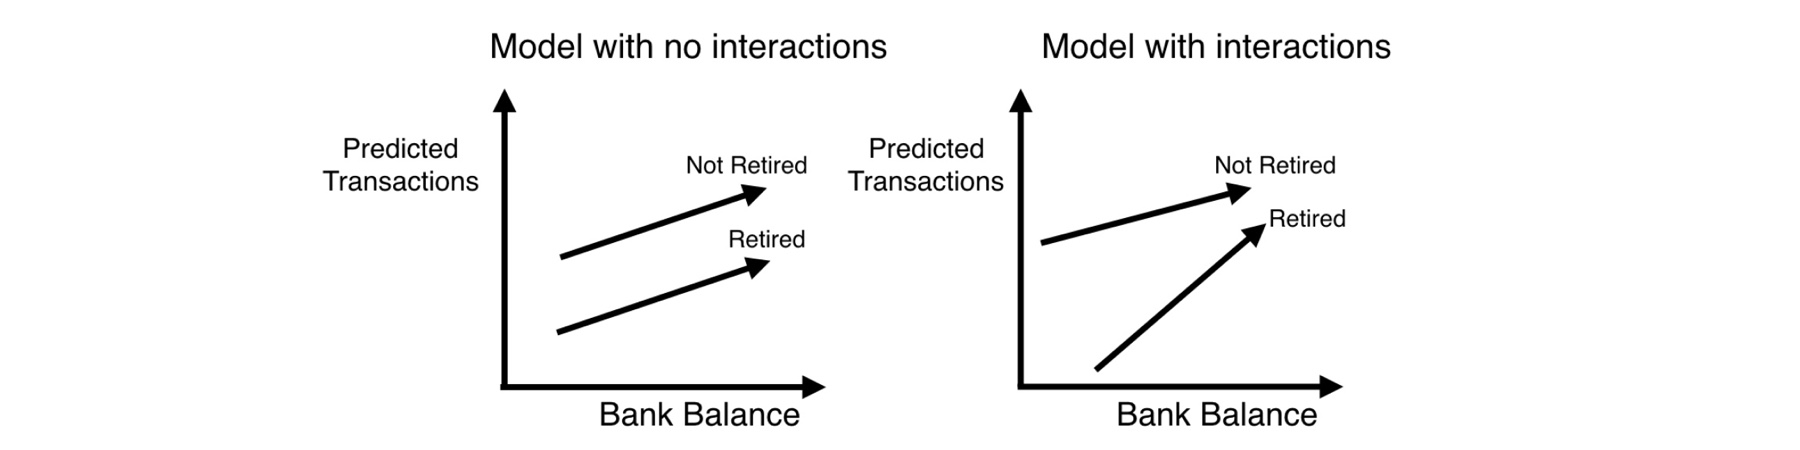
\includegraphics{../Figures/1. Example as seen by linear regression.jpg}
\caption{Example as seen by linear regression}
\end{figure}

    \hypertarget{note-2-interactions}{%
\subsection{\texorpdfstring{\texttt{{[}note-2{]}}
Interactions}{{[}note-2{]} Interactions}}\label{note-2-interactions}}

\begin{itemize}
\item
  Neural networks account for interactions really well.
\item
  Deep learning uses especially powerful neural networks:

  \begin{itemize}
  \item
    text
  \item
    images
  \item
    videos
  \item
    audio
  \item
    source code
  \end{itemize}
\end{itemize}

    \hypertarget{note-3-interactions-in-neural-network}{%
\subsection{\texorpdfstring{\texttt{{[}note-3{]}} Interactions in neural
network}{{[}note-3{]} Interactions in neural network}}\label{note-3-interactions-in-neural-network}}

\begin{figure}
\centering
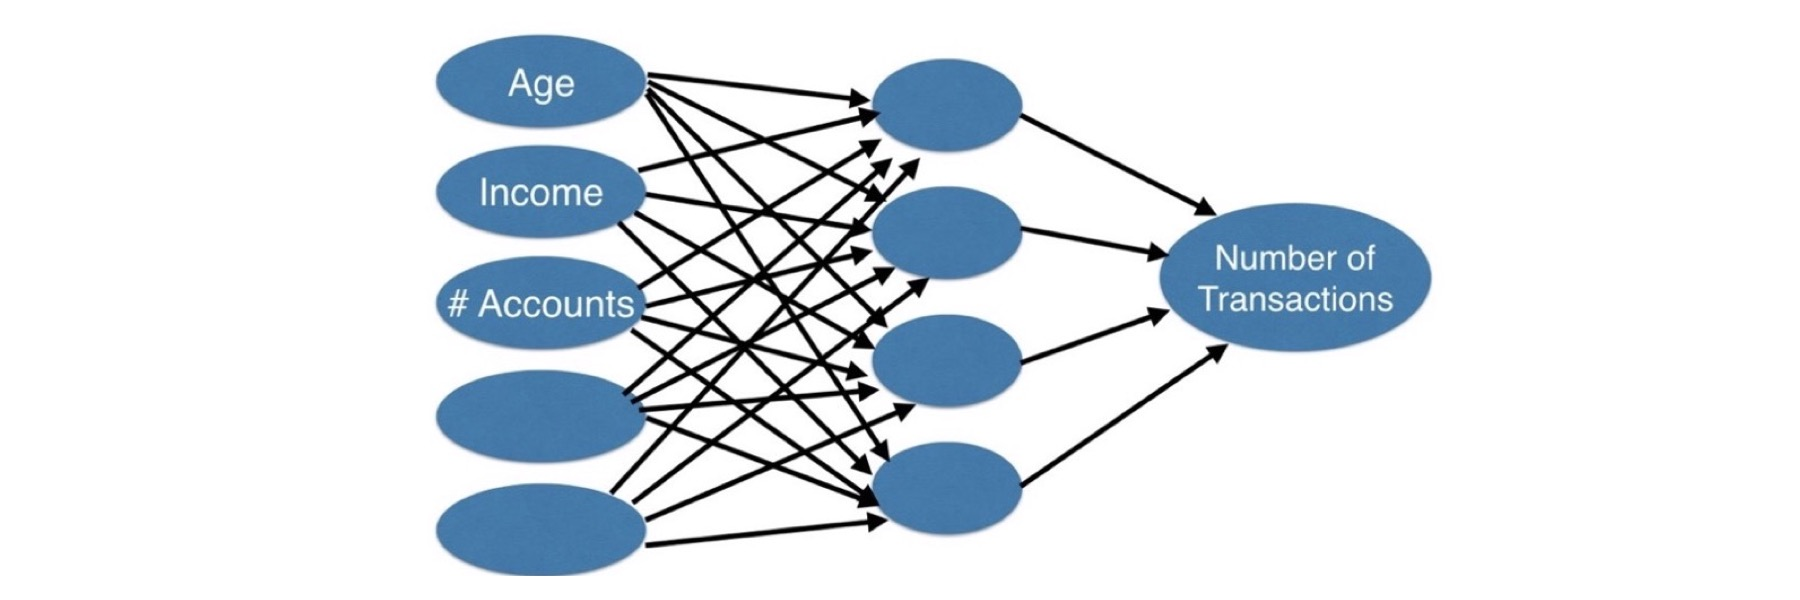
\includegraphics{../Figures/2. Interactions in neural network.jpg}
\caption{Interactions in neural network}
\end{figure}

    \hypertarget{quiz-1-comparing-neural-network-models-to-classical-regression-models}{%
\subsection{\texorpdfstring{\texttt{{[}quiz-1{]}} Comparing neural
network models to classical regression
models}{{[}quiz-1{]} Comparing neural network models to classical regression models}}\label{quiz-1-comparing-neural-network-models-to-classical-regression-models}}

\begin{itemize}
\item
  Which of the models in the diagrams has a greater ability to account
  for interactions?

  \begin{figure}
  \centering
  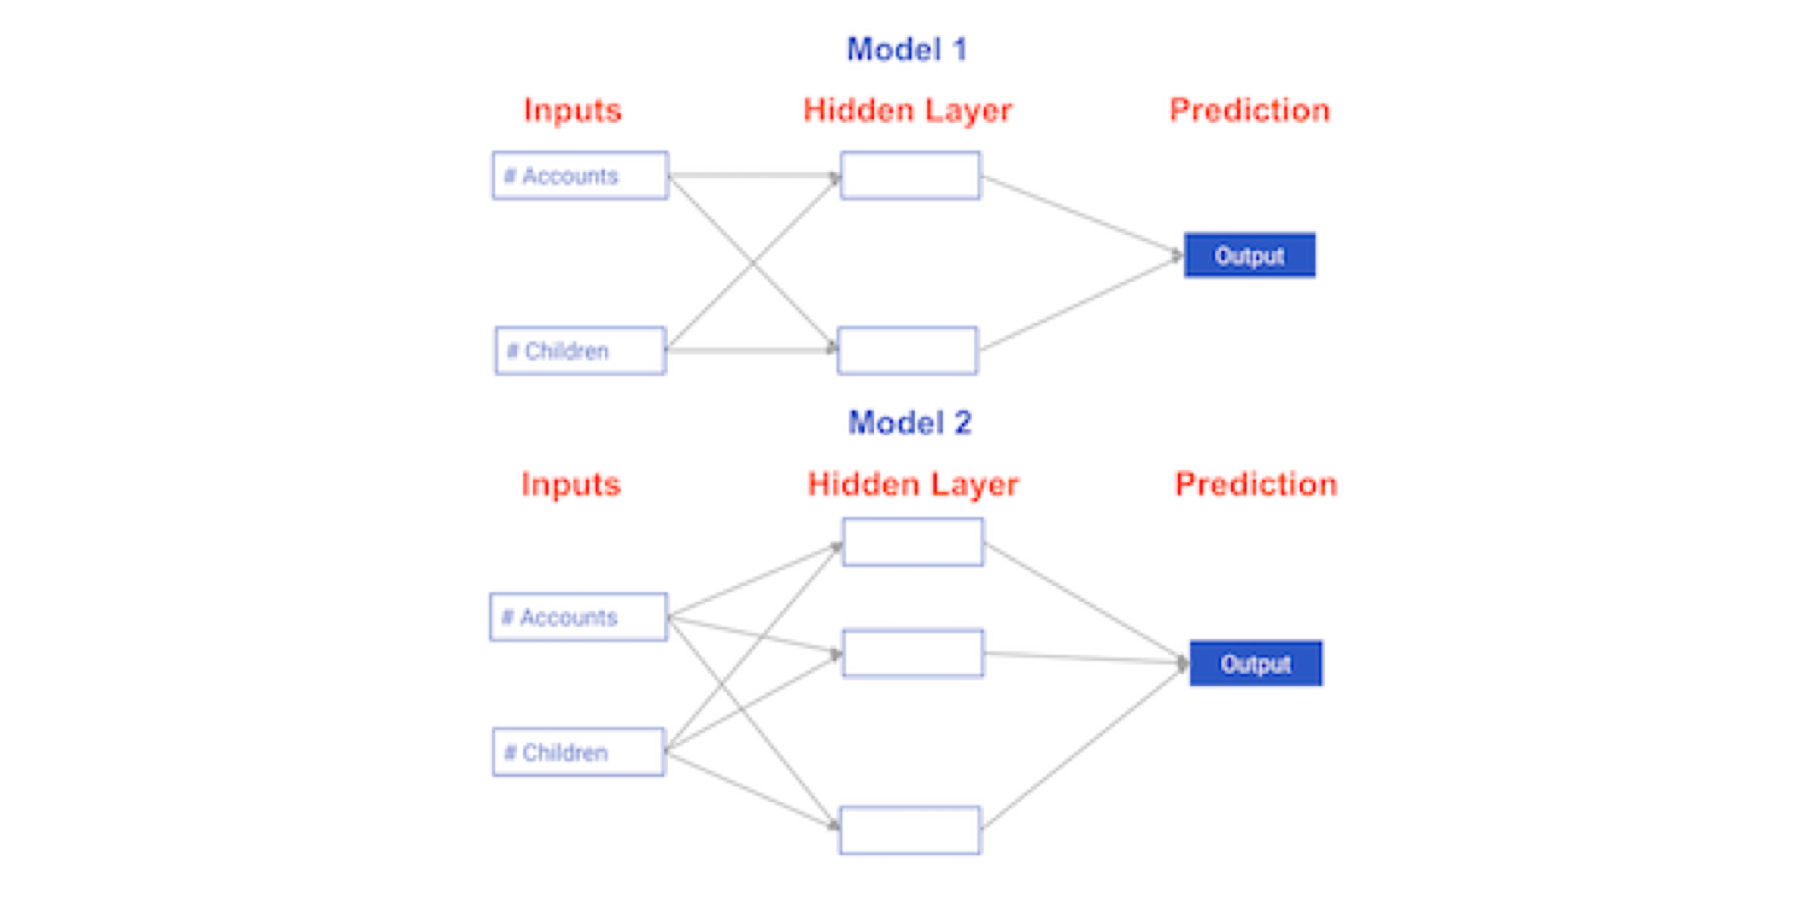
\includegraphics{../Figures/3. Comparing neural network models to classical regression models.png}
  \caption{Comparing neural network models to classical regression
  models}
  \end{figure}

  \(\Box\) Model 1.

  \(\boxtimes\) Model 2.

  \(\Box\) They are both the same.
\end{itemize}

    \hypertarget{forward-propagation}{%
\section{Forward propagation}\label{forward-propagation}}

    \hypertarget{note-1-forward-propagation}{%
\subsection{\texorpdfstring{\texttt{{[}note-1{]}} Forward
propagation}{{[}note-1{]} Forward propagation}}\label{note-1-forward-propagation}}

\begin{itemize}
\item
  Multiply - add process.
\item
  Dot product.
\item
  Propagate forward for one data point at a time.
\item
  Output is the prediction for that data point.
\end{itemize}

\begin{figure}
\centering
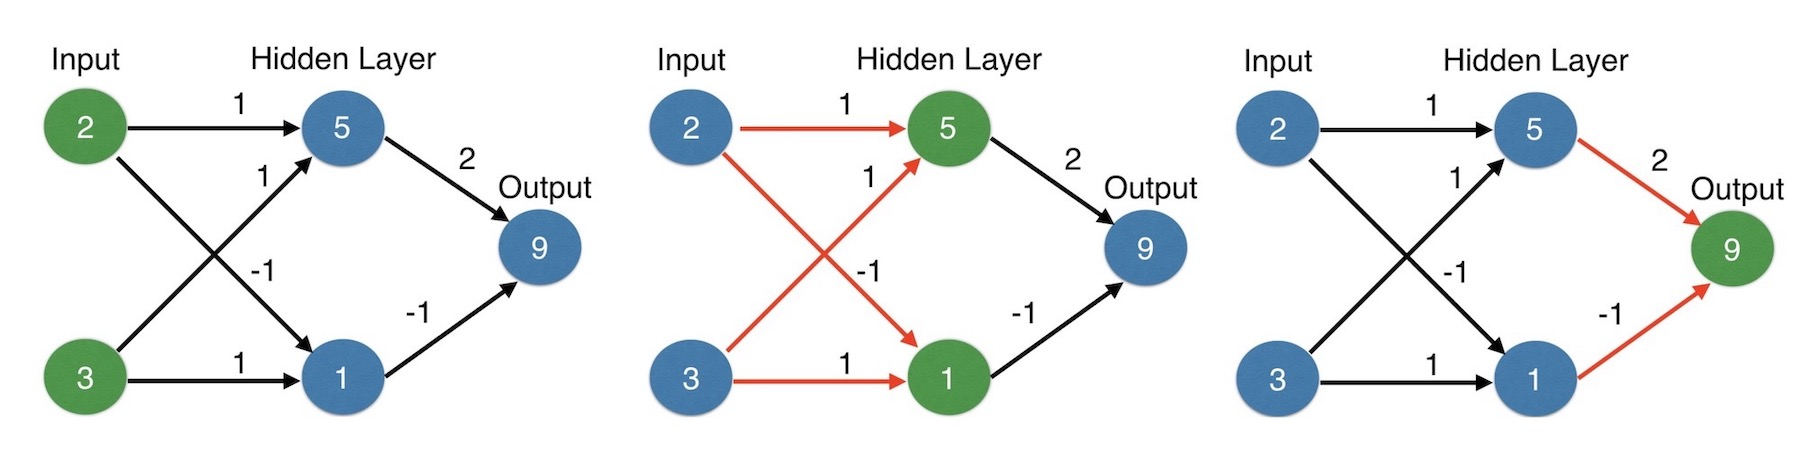
\includegraphics{../Figures/4. Forward propagation.jpg}
\caption{Forward propagation}
\end{figure}

    \hypertarget{code-1-forward-propagation}{%
\subsection{\texorpdfstring{\texttt{{[}code-1{]}} Forward
propagation}{{[}code-1{]} Forward propagation}}\label{code-1-forward-propagation}}

    \begin{tcolorbox}[breakable, size=fbox, boxrule=1pt, pad at break*=1mm,colback=cellbackground, colframe=cellborder]
\prompt{In}{incolor}{1}{\boxspacing}
\begin{Verbatim}[commandchars=\\\{\}]
\PY{k+kn}{import} \PY{n+nn}{numpy} \PY{k}{as} \PY{n+nn}{np}

\PY{n}{input\PYZus{}data} \PY{o}{=} \PY{n}{np}\PY{o}{.}\PY{n}{array}\PY{p}{(}\PY{p}{[}\PY{l+m+mi}{2}\PY{p}{,} \PY{l+m+mi}{3}\PY{p}{]}\PY{p}{)}
\PY{n}{weights} \PY{o}{=} \PY{p}{\PYZob{}}
    \PY{l+s+s1}{\PYZsq{}}\PY{l+s+s1}{node\PYZus{}0}\PY{l+s+s1}{\PYZsq{}}\PY{p}{:} \PY{n}{np}\PY{o}{.}\PY{n}{array}\PY{p}{(}\PY{p}{[}\PY{l+m+mi}{1}\PY{p}{,} \PY{l+m+mi}{1}\PY{p}{]}\PY{p}{)}\PY{p}{,}
    \PY{l+s+s1}{\PYZsq{}}\PY{l+s+s1}{node\PYZus{}1}\PY{l+s+s1}{\PYZsq{}}\PY{p}{:} \PY{n}{np}\PY{o}{.}\PY{n}{array}\PY{p}{(}\PY{p}{[}\PY{o}{\PYZhy{}}\PY{l+m+mi}{1}\PY{p}{,} \PY{l+m+mi}{1}\PY{p}{]}\PY{p}{)}\PY{p}{,}
    \PY{l+s+s1}{\PYZsq{}}\PY{l+s+s1}{output}\PY{l+s+s1}{\PYZsq{}}\PY{p}{:} \PY{n}{np}\PY{o}{.}\PY{n}{array}\PY{p}{(}\PY{p}{[}\PY{l+m+mi}{2}\PY{p}{,} \PY{o}{\PYZhy{}}\PY{l+m+mi}{1}\PY{p}{]}\PY{p}{)}
\PY{p}{\PYZcb{}}
\PY{n}{node\PYZus{}0\PYZus{}value} \PY{o}{=} \PY{p}{(}\PY{n}{input\PYZus{}data} \PY{o}{*} \PY{n}{weights}\PY{p}{[}\PY{l+s+s1}{\PYZsq{}}\PY{l+s+s1}{node\PYZus{}0}\PY{l+s+s1}{\PYZsq{}}\PY{p}{]}\PY{p}{)}\PY{o}{.}\PY{n}{sum}\PY{p}{(}\PY{p}{)}
\PY{n}{node\PYZus{}1\PYZus{}value} \PY{o}{=} \PY{p}{(}\PY{n}{input\PYZus{}data} \PY{o}{*} \PY{n}{weights}\PY{p}{[}\PY{l+s+s1}{\PYZsq{}}\PY{l+s+s1}{node\PYZus{}1}\PY{l+s+s1}{\PYZsq{}}\PY{p}{]}\PY{p}{)}\PY{o}{.}\PY{n}{sum}\PY{p}{(}\PY{p}{)}

\PY{n}{hidden\PYZus{}layer\PYZus{}values} \PY{o}{=} \PY{n}{np}\PY{o}{.}\PY{n}{array}\PY{p}{(}\PY{p}{[}\PY{n}{node\PYZus{}0\PYZus{}value}\PY{p}{,} \PY{n}{node\PYZus{}1\PYZus{}value}\PY{p}{]}\PY{p}{)}
\PY{n+nb}{print}\PY{p}{(}\PY{n}{hidden\PYZus{}layer\PYZus{}values}\PY{p}{)}
\end{Verbatim}
\end{tcolorbox}

    \begin{Verbatim}[commandchars=\\\{\}]
[5 1]
    \end{Verbatim}

    \begin{tcolorbox}[breakable, size=fbox, boxrule=1pt, pad at break*=1mm,colback=cellbackground, colframe=cellborder]
\prompt{In}{incolor}{2}{\boxspacing}
\begin{Verbatim}[commandchars=\\\{\}]
\PY{n}{output} \PY{o}{=} \PY{p}{(}\PY{n}{hidden\PYZus{}layer\PYZus{}values} \PY{o}{*} \PY{n}{weights}\PY{p}{[}\PY{l+s+s1}{\PYZsq{}}\PY{l+s+s1}{output}\PY{l+s+s1}{\PYZsq{}}\PY{p}{]}\PY{p}{)}\PY{o}{.}\PY{n}{sum}\PY{p}{(}\PY{p}{)}
\PY{n+nb}{print}\PY{p}{(}\PY{n}{output}\PY{p}{)}
\end{Verbatim}
\end{tcolorbox}

    \begin{Verbatim}[commandchars=\\\{\}]
9
    \end{Verbatim}

    \hypertarget{task-1-coding-the-forward-propagation-algorithm}{%
\subsection{\texorpdfstring{\texttt{{[}task-1{]}} Coding the forward
propagation
algorithm}{{[}task-1{]} Coding the forward propagation algorithm}}\label{task-1-coding-the-forward-propagation-algorithm}}

\(\blacktriangleright\) \textbf{Task diagram}

\begin{figure}
\centering

\includegraphics{../Figures/5. Coding the forward propagation algorithm.png}
\caption{Coding the forward propagation algorithm}
\end{figure}

    \(\blacktriangleright\) \textbf{Package pre-loading}

    \begin{tcolorbox}[breakable, size=fbox, boxrule=1pt, pad at break*=1mm,colback=cellbackground, colframe=cellborder]
\prompt{In}{incolor}{3}{\boxspacing}
\begin{Verbatim}[commandchars=\\\{\}]
\PY{k+kn}{import} \PY{n+nn}{numpy} \PY{k}{as} \PY{n+nn}{np}
\end{Verbatim}
\end{tcolorbox}

    \(\blacktriangleright\) \textbf{Data pre-loading}

    \begin{tcolorbox}[breakable, size=fbox, boxrule=1pt, pad at break*=1mm,colback=cellbackground, colframe=cellborder]
\prompt{In}{incolor}{4}{\boxspacing}
\begin{Verbatim}[commandchars=\\\{\}]
\PY{n}{input\PYZus{}data} \PY{o}{=} \PY{n}{np}\PY{o}{.}\PY{n}{array}\PY{p}{(}\PY{p}{[}\PY{l+m+mi}{3}\PY{p}{,} \PY{l+m+mi}{5}\PY{p}{]}\PY{p}{)}

\PY{n}{weights} \PY{o}{=} \PY{p}{\PYZob{}}
    \PY{l+s+s1}{\PYZsq{}}\PY{l+s+s1}{node\PYZus{}0}\PY{l+s+s1}{\PYZsq{}}\PY{p}{:} \PY{n}{np}\PY{o}{.}\PY{n}{array}\PY{p}{(}\PY{p}{[}\PY{l+m+mi}{2}\PY{p}{,} \PY{l+m+mi}{4}\PY{p}{]}\PY{p}{)}\PY{p}{,}
    \PY{l+s+s1}{\PYZsq{}}\PY{l+s+s1}{node\PYZus{}1}\PY{l+s+s1}{\PYZsq{}}\PY{p}{:} \PY{n}{np}\PY{o}{.}\PY{n}{array}\PY{p}{(}\PY{p}{[}\PY{l+m+mi}{4}\PY{p}{,} \PY{o}{\PYZhy{}}\PY{l+m+mi}{5}\PY{p}{]}\PY{p}{)}\PY{p}{,}
    \PY{l+s+s1}{\PYZsq{}}\PY{l+s+s1}{output}\PY{l+s+s1}{\PYZsq{}}\PY{p}{:} \PY{n}{np}\PY{o}{.}\PY{n}{array}\PY{p}{(}\PY{p}{[}\PY{l+m+mi}{2}\PY{p}{,} \PY{l+m+mi}{7}\PY{p}{]}\PY{p}{)}
\PY{p}{\PYZcb{}}
\end{Verbatim}
\end{tcolorbox}

    \(\blacktriangleright\) \textbf{Task practice}

    \begin{tcolorbox}[breakable, size=fbox, boxrule=1pt, pad at break*=1mm,colback=cellbackground, colframe=cellborder]
\prompt{In}{incolor}{5}{\boxspacing}
\begin{Verbatim}[commandchars=\\\{\}]
\PY{c+c1}{\PYZsh{} Calculate node 0 value: node\PYZus{}0\PYZus{}value}
\PY{n}{node\PYZus{}0\PYZus{}value} \PY{o}{=} \PY{p}{(}\PY{n}{input\PYZus{}data} \PY{o}{*} \PY{n}{weights}\PY{p}{[}\PY{l+s+s1}{\PYZsq{}}\PY{l+s+s1}{node\PYZus{}0}\PY{l+s+s1}{\PYZsq{}}\PY{p}{]}\PY{p}{)}\PY{o}{.}\PY{n}{sum}\PY{p}{(}\PY{p}{)}

\PY{c+c1}{\PYZsh{} Calculate node 1 value: node\PYZus{}1\PYZus{}value}
\PY{n}{node\PYZus{}1\PYZus{}value} \PY{o}{=} \PY{p}{(}\PY{n}{input\PYZus{}data} \PY{o}{*} \PY{n}{weights}\PY{p}{[}\PY{l+s+s1}{\PYZsq{}}\PY{l+s+s1}{node\PYZus{}1}\PY{l+s+s1}{\PYZsq{}}\PY{p}{]}\PY{p}{)}\PY{o}{.}\PY{n}{sum}\PY{p}{(}\PY{p}{)}

\PY{c+c1}{\PYZsh{} Put node values into array: hidden\PYZus{}layer\PYZus{}outputs}
\PY{n}{hidden\PYZus{}layer\PYZus{}outputs} \PY{o}{=} \PY{n}{np}\PY{o}{.}\PY{n}{array}\PY{p}{(}\PY{p}{[}\PY{n}{node\PYZus{}0\PYZus{}value}\PY{p}{,} \PY{n}{node\PYZus{}1\PYZus{}value}\PY{p}{]}\PY{p}{)}

\PY{c+c1}{\PYZsh{} Calculate output: output}
\PY{n}{output} \PY{o}{=} \PY{p}{(}\PY{n}{hidden\PYZus{}layer\PYZus{}outputs} \PY{o}{*} \PY{n}{weights}\PY{p}{[}\PY{l+s+s1}{\PYZsq{}}\PY{l+s+s1}{output}\PY{l+s+s1}{\PYZsq{}}\PY{p}{]}\PY{p}{)}\PY{o}{.}\PY{n}{sum}\PY{p}{(}\PY{p}{)}

\PY{c+c1}{\PYZsh{} Print output}
\PY{n+nb}{print}\PY{p}{(}\PY{n}{output}\PY{p}{)}
\end{Verbatim}
\end{tcolorbox}

    \begin{Verbatim}[commandchars=\\\{\}]
-39
    \end{Verbatim}

    \hypertarget{activation-functions}{%
\section{Activation functions}\label{activation-functions}}

    \hypertarget{note-1-linear-vs.-nonlinear-functions}{%
\subsection{\texorpdfstring{\texttt{{[}note-1{]}} Linear vs.~nonlinear
functions}{{[}note-1{]} Linear vs.~nonlinear functions}}\label{note-1-linear-vs.-nonlinear-functions}}

\begin{figure}
\centering
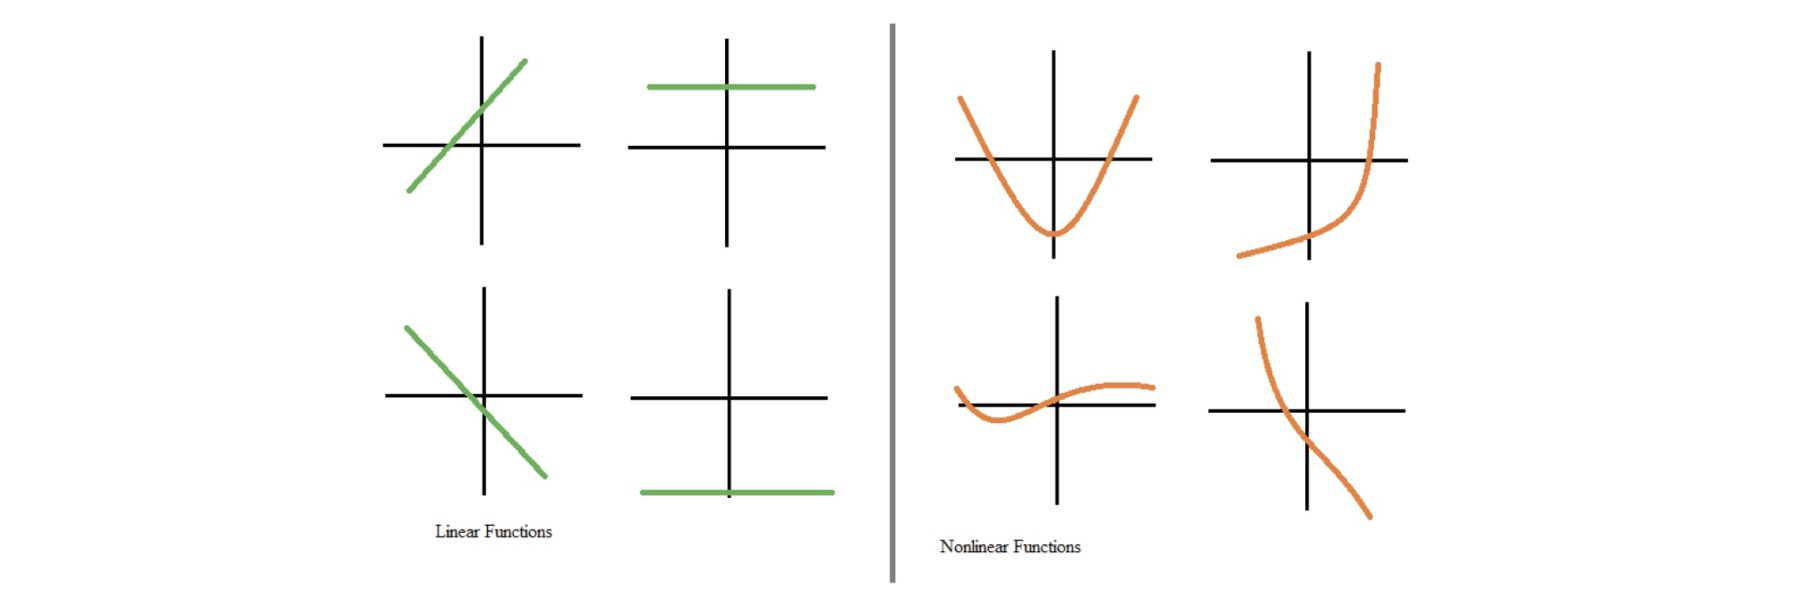
\includegraphics{../Figures/6. Linear vs. nonlinear functions.jpg}
\caption{Linear vs.~nonlinear functions}
\end{figure}

    \hypertarget{note-2-activation-functions}{%
\subsection{\texorpdfstring{\texttt{{[}note-2{]}} Activation
functions}{{[}note-2{]} Activation functions}}\label{note-2-activation-functions}}

\begin{itemize}
\tightlist
\item
  Activation functions are applied to node inputs to produce node
  output.
\end{itemize}

\begin{figure}
\centering
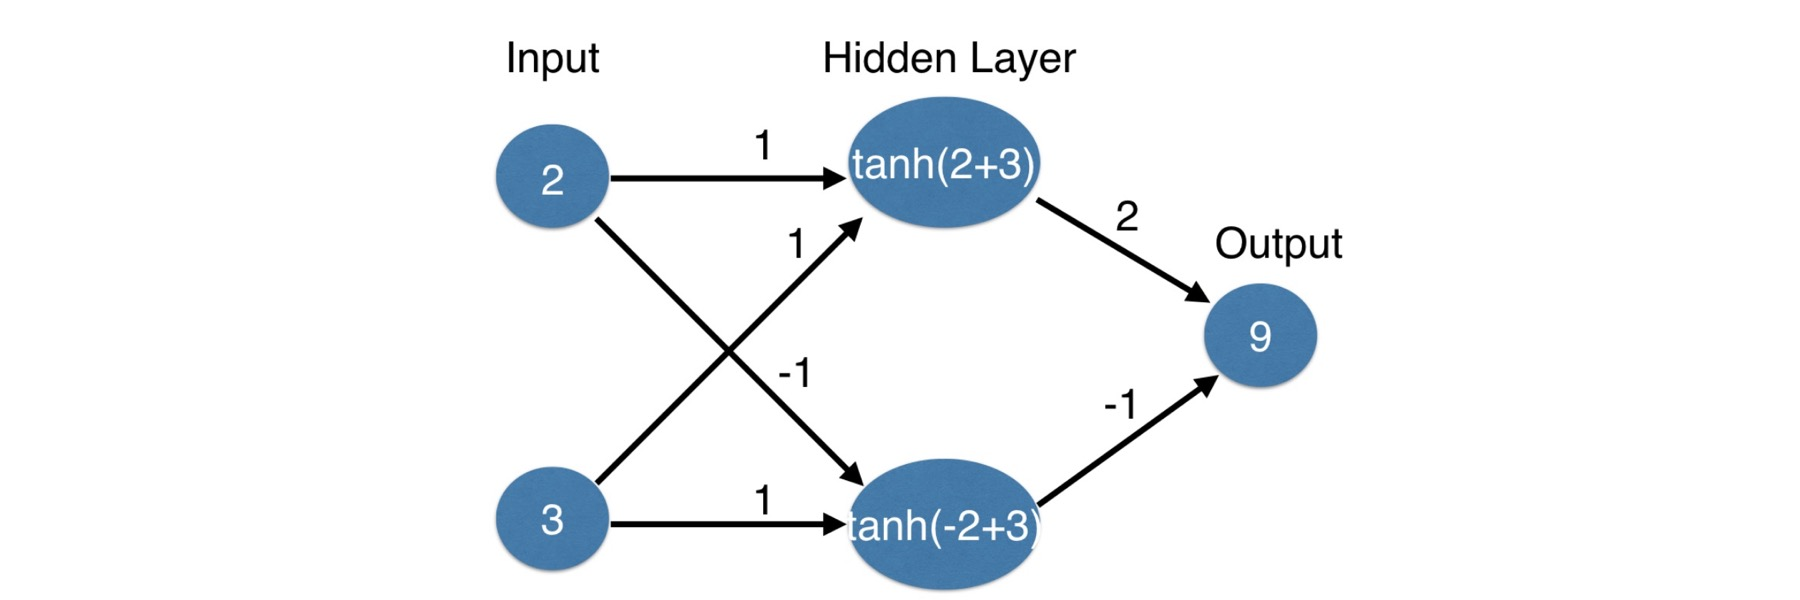
\includegraphics{../Figures/7. Activation functions.jpg}
\caption{Activation functions}
\end{figure}

    \hypertarget{note-3-relu-rectified-linear-activation}{%
\subsection{\texorpdfstring{\texttt{{[}note-3{]}} ReLU (Rectified Linear
Activation)}{{[}note-3{]} ReLU (Rectified Linear Activation)}}\label{note-3-relu-rectified-linear-activation}}

\begin{figure}
\centering
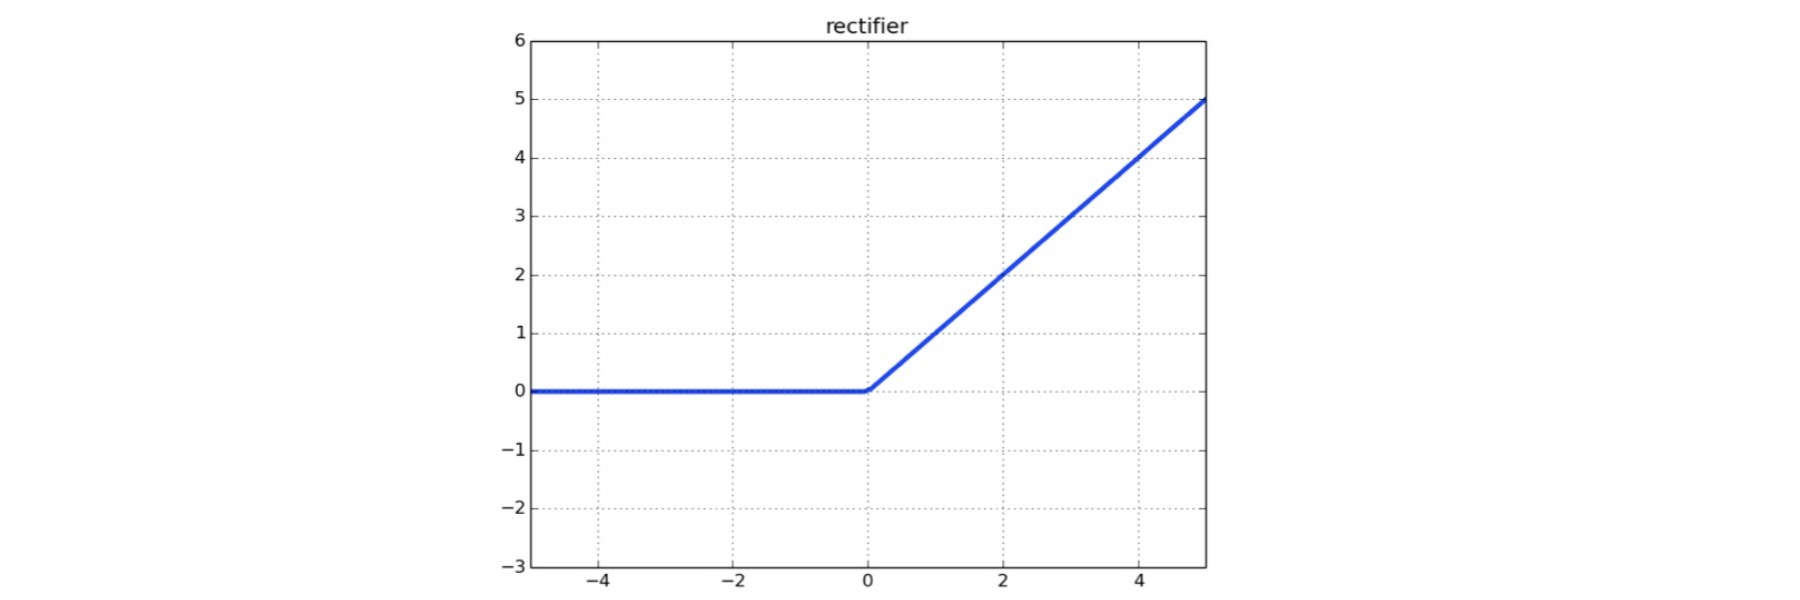
\includegraphics{../Figures/8. ReLU (Rectified Linear Activation).jpg}
\caption{ReLU (Rectified Linear Activation)}
\end{figure}

\begin{equation*}
    RELU(x)\ =\
    \begin{cases}
        \begin{aligned}
            0\ if\ x\ <   \ 0\\
            x\ if\ x\ \geq\ 0  
        \end{aligned}
    \end{cases}
\end{equation*}

    \hypertarget{code-1-activation-functions}{%
\subsection{\texorpdfstring{\texttt{{[}code-1{]}} Activation
functions}{{[}code-1{]} Activation functions}}\label{code-1-activation-functions}}

    \begin{tcolorbox}[breakable, size=fbox, boxrule=1pt, pad at break*=1mm,colback=cellbackground, colframe=cellborder]
\prompt{In}{incolor}{6}{\boxspacing}
\begin{Verbatim}[commandchars=\\\{\}]
\PY{k+kn}{import} \PY{n+nn}{numpy} \PY{k}{as} \PY{n+nn}{np}

\PY{n}{input\PYZus{}data} \PY{o}{=} \PY{n}{np}\PY{o}{.}\PY{n}{array}\PY{p}{(}\PY{p}{[}\PY{o}{\PYZhy{}}\PY{l+m+mi}{1}\PY{p}{,} \PY{l+m+mi}{2}\PY{p}{]}\PY{p}{)}
\PY{n}{weights} \PY{o}{=} \PY{p}{\PYZob{}}
    \PY{l+s+s1}{\PYZsq{}}\PY{l+s+s1}{node\PYZus{}0}\PY{l+s+s1}{\PYZsq{}}\PY{p}{:} \PY{n}{np}\PY{o}{.}\PY{n}{array}\PY{p}{(}\PY{p}{[}\PY{l+m+mi}{3}\PY{p}{,} \PY{l+m+mi}{3}\PY{p}{]}\PY{p}{)}\PY{p}{,}
    \PY{l+s+s1}{\PYZsq{}}\PY{l+s+s1}{node\PYZus{}1}\PY{l+s+s1}{\PYZsq{}}\PY{p}{:} \PY{n}{np}\PY{o}{.}\PY{n}{array}\PY{p}{(}\PY{p}{[}\PY{l+m+mi}{1}\PY{p}{,} \PY{l+m+mi}{5}\PY{p}{]}\PY{p}{)}\PY{p}{,}
    \PY{l+s+s1}{\PYZsq{}}\PY{l+s+s1}{output}\PY{l+s+s1}{\PYZsq{}}\PY{p}{:} \PY{n}{np}\PY{o}{.}\PY{n}{array}\PY{p}{(}\PY{p}{[}\PY{l+m+mi}{2}\PY{p}{,} \PY{o}{\PYZhy{}}\PY{l+m+mi}{1}\PY{p}{]}\PY{p}{)}
\PY{p}{\PYZcb{}}
\PY{n}{node\PYZus{}0\PYZus{}input} \PY{o}{=} \PY{p}{(}\PY{n}{input\PYZus{}data} \PY{o}{*} \PY{n}{weights}\PY{p}{[}\PY{l+s+s1}{\PYZsq{}}\PY{l+s+s1}{node\PYZus{}0}\PY{l+s+s1}{\PYZsq{}}\PY{p}{]}\PY{p}{)}\PY{o}{.}\PY{n}{sum}\PY{p}{(}\PY{p}{)}
\PY{n}{node\PYZus{}0\PYZus{}output} \PY{o}{=} \PY{n}{np}\PY{o}{.}\PY{n}{tanh}\PY{p}{(}\PY{n}{node\PYZus{}0\PYZus{}input}\PY{p}{)}
\PY{n}{node\PYZus{}1\PYZus{}input} \PY{o}{=} \PY{p}{(}\PY{n}{input\PYZus{}data} \PY{o}{*} \PY{n}{weights}\PY{p}{[}\PY{l+s+s1}{\PYZsq{}}\PY{l+s+s1}{node\PYZus{}1}\PY{l+s+s1}{\PYZsq{}}\PY{p}{]}\PY{p}{)}\PY{o}{.}\PY{n}{sum}\PY{p}{(}\PY{p}{)}
\PY{n}{node\PYZus{}1\PYZus{}output} \PY{o}{=} \PY{n}{np}\PY{o}{.}\PY{n}{tanh}\PY{p}{(}\PY{n}{node\PYZus{}1\PYZus{}input}\PY{p}{)}
\PY{n}{hidden\PYZus{}layer\PYZus{}outputs} \PY{o}{=} \PY{n}{np}\PY{o}{.}\PY{n}{array}\PY{p}{(}\PY{p}{[}\PY{n}{node\PYZus{}0\PYZus{}output}\PY{p}{,} \PY{n}{node\PYZus{}1\PYZus{}output}\PY{p}{]}\PY{p}{)}
\PY{n}{output} \PY{o}{=} \PY{p}{(}\PY{n}{hidden\PYZus{}layer\PYZus{}outputs} \PY{o}{*} \PY{n}{weights}\PY{p}{[}\PY{l+s+s1}{\PYZsq{}}\PY{l+s+s1}{output}\PY{l+s+s1}{\PYZsq{}}\PY{p}{]}\PY{p}{)}\PY{o}{.}\PY{n}{sum}\PY{p}{(}\PY{p}{)}

\PY{n+nb}{print}\PY{p}{(}\PY{n}{output}\PY{p}{)}
\end{Verbatim}
\end{tcolorbox}

    \begin{Verbatim}[commandchars=\\\{\}]
0.9901095378334199
    \end{Verbatim}

    \hypertarget{task-1-the-rectified-linear-activation-function}{%
\subsection{\texorpdfstring{\texttt{{[}task-1{]}} The rectified linear
activation
function}{{[}task-1{]} The rectified linear activation function}}\label{task-1-the-rectified-linear-activation-function}}

\(\blacktriangleright\) \textbf{Package pre-loading}

    \begin{tcolorbox}[breakable, size=fbox, boxrule=1pt, pad at break*=1mm,colback=cellbackground, colframe=cellborder]
\prompt{In}{incolor}{7}{\boxspacing}
\begin{Verbatim}[commandchars=\\\{\}]
\PY{k+kn}{import} \PY{n+nn}{numpy} \PY{k}{as} \PY{n+nn}{np}
\end{Verbatim}
\end{tcolorbox}

    \(\blacktriangleright\) \textbf{Data pre-loading}

    \begin{tcolorbox}[breakable, size=fbox, boxrule=1pt, pad at break*=1mm,colback=cellbackground, colframe=cellborder]
\prompt{In}{incolor}{8}{\boxspacing}
\begin{Verbatim}[commandchars=\\\{\}]
\PY{n}{input\PYZus{}data} \PY{o}{=} \PY{n}{np}\PY{o}{.}\PY{n}{array}\PY{p}{(}\PY{p}{[}\PY{l+m+mi}{3}\PY{p}{,} \PY{l+m+mi}{5}\PY{p}{]}\PY{p}{)}

\PY{n}{weights} \PY{o}{=} \PY{p}{\PYZob{}}
    \PY{l+s+s1}{\PYZsq{}}\PY{l+s+s1}{node\PYZus{}0}\PY{l+s+s1}{\PYZsq{}}\PY{p}{:} \PY{n}{np}\PY{o}{.}\PY{n}{array}\PY{p}{(}\PY{p}{[}\PY{l+m+mi}{2}\PY{p}{,} \PY{l+m+mi}{4}\PY{p}{]}\PY{p}{)}\PY{p}{,}
    \PY{l+s+s1}{\PYZsq{}}\PY{l+s+s1}{node\PYZus{}1}\PY{l+s+s1}{\PYZsq{}}\PY{p}{:} \PY{n}{np}\PY{o}{.}\PY{n}{array}\PY{p}{(}\PY{p}{[}\PY{l+m+mi}{4}\PY{p}{,} \PY{o}{\PYZhy{}}\PY{l+m+mi}{5}\PY{p}{]}\PY{p}{)}\PY{p}{,}
    \PY{l+s+s1}{\PYZsq{}}\PY{l+s+s1}{output}\PY{l+s+s1}{\PYZsq{}}\PY{p}{:} \PY{n}{np}\PY{o}{.}\PY{n}{array}\PY{p}{(}\PY{p}{[}\PY{l+m+mi}{2}\PY{p}{,} \PY{l+m+mi}{7}\PY{p}{]}\PY{p}{)}
\PY{p}{\PYZcb{}}
\end{Verbatim}
\end{tcolorbox}

    \(\blacktriangleright\) \textbf{Task practice}

    \begin{tcolorbox}[breakable, size=fbox, boxrule=1pt, pad at break*=1mm,colback=cellbackground, colframe=cellborder]
\prompt{In}{incolor}{9}{\boxspacing}
\begin{Verbatim}[commandchars=\\\{\}]
\PY{k}{def} \PY{n+nf}{relu}\PY{p}{(}\PY{n+nb}{input}\PY{p}{)}\PY{p}{:}
    \PY{l+s+sd}{\PYZsq{}\PYZsq{}\PYZsq{}Define your relu activation function here\PYZsq{}\PYZsq{}\PYZsq{}}
    \PY{c+c1}{\PYZsh{} Calculate the value for the output of the relu function: output}
    \PY{n}{output} \PY{o}{=} \PY{n+nb}{max}\PY{p}{(}\PY{l+m+mi}{0}\PY{p}{,} \PY{n+nb}{input}\PY{p}{)}

    \PY{c+c1}{\PYZsh{} Return the value just calculated}
    \PY{k}{return} \PY{p}{(}\PY{n}{output}\PY{p}{)}


\PY{c+c1}{\PYZsh{} Calculate node 0 value: node\PYZus{}0\PYZus{}output}
\PY{n}{node\PYZus{}0\PYZus{}input} \PY{o}{=} \PY{p}{(}\PY{n}{input\PYZus{}data} \PY{o}{*} \PY{n}{weights}\PY{p}{[}\PY{l+s+s1}{\PYZsq{}}\PY{l+s+s1}{node\PYZus{}0}\PY{l+s+s1}{\PYZsq{}}\PY{p}{]}\PY{p}{)}\PY{o}{.}\PY{n}{sum}\PY{p}{(}\PY{p}{)}
\PY{n}{node\PYZus{}0\PYZus{}output} \PY{o}{=} \PY{n}{relu}\PY{p}{(}\PY{n}{node\PYZus{}0\PYZus{}input}\PY{p}{)}

\PY{c+c1}{\PYZsh{} Calculate node 1 value: node\PYZus{}1\PYZus{}output}
\PY{n}{node\PYZus{}1\PYZus{}input} \PY{o}{=} \PY{p}{(}\PY{n}{input\PYZus{}data} \PY{o}{*} \PY{n}{weights}\PY{p}{[}\PY{l+s+s1}{\PYZsq{}}\PY{l+s+s1}{node\PYZus{}1}\PY{l+s+s1}{\PYZsq{}}\PY{p}{]}\PY{p}{)}\PY{o}{.}\PY{n}{sum}\PY{p}{(}\PY{p}{)}
\PY{n}{node\PYZus{}1\PYZus{}output} \PY{o}{=} \PY{n}{relu}\PY{p}{(}\PY{n}{node\PYZus{}1\PYZus{}input}\PY{p}{)}

\PY{c+c1}{\PYZsh{} Put node values into array: hidden\PYZus{}layer\PYZus{}outputs}
\PY{n}{hidden\PYZus{}layer\PYZus{}outputs} \PY{o}{=} \PY{n}{np}\PY{o}{.}\PY{n}{array}\PY{p}{(}\PY{p}{[}\PY{n}{node\PYZus{}0\PYZus{}output}\PY{p}{,} \PY{n}{node\PYZus{}1\PYZus{}output}\PY{p}{]}\PY{p}{)}

\PY{c+c1}{\PYZsh{} Calculate model output (do not apply relu)}
\PY{n}{model\PYZus{}output} \PY{o}{=} \PY{p}{(}\PY{n}{hidden\PYZus{}layer\PYZus{}outputs} \PY{o}{*} \PY{n}{weights}\PY{p}{[}\PY{l+s+s1}{\PYZsq{}}\PY{l+s+s1}{output}\PY{l+s+s1}{\PYZsq{}}\PY{p}{]}\PY{p}{)}\PY{o}{.}\PY{n}{sum}\PY{p}{(}\PY{p}{)}

\PY{c+c1}{\PYZsh{} Print model output}
\PY{n+nb}{print}\PY{p}{(}\PY{n}{model\PYZus{}output}\PY{p}{)}
\end{Verbatim}
\end{tcolorbox}

    \begin{Verbatim}[commandchars=\\\{\}]
52
    \end{Verbatim}

    \hypertarget{task-2-applying-the-network-to-many-observationsrows-of-data}{%
\subsection{\texorpdfstring{\texttt{{[}task-2{]}} Applying the network
to many observations/rows of
data}{{[}task-2{]} Applying the network to many observations/rows of data}}\label{task-2-applying-the-network-to-many-observationsrows-of-data}}

    \(\blacktriangleright\) \textbf{Data pre-loading}

    \begin{tcolorbox}[breakable, size=fbox, boxrule=1pt, pad at break*=1mm,colback=cellbackground, colframe=cellborder]
\prompt{In}{incolor}{10}{\boxspacing}
\begin{Verbatim}[commandchars=\\\{\}]
\PY{n}{input\PYZus{}data} \PY{o}{=} \PY{p}{[}
    \PY{n}{np}\PY{o}{.}\PY{n}{array}\PY{p}{(}\PY{p}{[}\PY{l+m+mi}{3}\PY{p}{,} \PY{l+m+mi}{5}\PY{p}{]}\PY{p}{)}\PY{p}{,}
    \PY{n}{np}\PY{o}{.}\PY{n}{array}\PY{p}{(}\PY{p}{[}\PY{l+m+mi}{1}\PY{p}{,} \PY{o}{\PYZhy{}}\PY{l+m+mi}{1}\PY{p}{]}\PY{p}{)}\PY{p}{,}
    \PY{n}{np}\PY{o}{.}\PY{n}{array}\PY{p}{(}\PY{p}{[}\PY{l+m+mi}{0}\PY{p}{,} \PY{l+m+mi}{0}\PY{p}{]}\PY{p}{)}\PY{p}{,}
    \PY{n}{np}\PY{o}{.}\PY{n}{array}\PY{p}{(}\PY{p}{[}\PY{l+m+mi}{8}\PY{p}{,} \PY{l+m+mi}{4}\PY{p}{]}\PY{p}{)}
\PY{p}{]}
\end{Verbatim}
\end{tcolorbox}

    \(\blacktriangleright\) \textbf{Task practice}

    \begin{tcolorbox}[breakable, size=fbox, boxrule=1pt, pad at break*=1mm,colback=cellbackground, colframe=cellborder]
\prompt{In}{incolor}{11}{\boxspacing}
\begin{Verbatim}[commandchars=\\\{\}]
\PY{c+c1}{\PYZsh{} Define predict\PYZus{}with\PYZus{}network()}
\PY{k}{def} \PY{n+nf}{predict\PYZus{}with\PYZus{}network}\PY{p}{(}\PY{n}{input\PYZus{}data\PYZus{}row}\PY{p}{,} \PY{n}{weights}\PY{p}{)}\PY{p}{:}

    \PY{c+c1}{\PYZsh{} Calculate node 0 value}
    \PY{n}{node\PYZus{}0\PYZus{}input} \PY{o}{=} \PY{p}{(}\PY{n}{input\PYZus{}data\PYZus{}row} \PY{o}{*} \PY{n}{weights}\PY{p}{[}\PY{l+s+s1}{\PYZsq{}}\PY{l+s+s1}{node\PYZus{}0}\PY{l+s+s1}{\PYZsq{}}\PY{p}{]}\PY{p}{)}\PY{o}{.}\PY{n}{sum}\PY{p}{(}\PY{p}{)}
    \PY{n}{node\PYZus{}0\PYZus{}output} \PY{o}{=} \PY{n}{relu}\PY{p}{(}\PY{n}{node\PYZus{}0\PYZus{}input}\PY{p}{)}

    \PY{c+c1}{\PYZsh{} Calculate node 1 value}
    \PY{n}{node\PYZus{}1\PYZus{}input} \PY{o}{=} \PY{p}{(}\PY{n}{input\PYZus{}data\PYZus{}row} \PY{o}{*} \PY{n}{weights}\PY{p}{[}\PY{l+s+s1}{\PYZsq{}}\PY{l+s+s1}{node\PYZus{}1}\PY{l+s+s1}{\PYZsq{}}\PY{p}{]}\PY{p}{)}\PY{o}{.}\PY{n}{sum}\PY{p}{(}\PY{p}{)}
    \PY{n}{node\PYZus{}1\PYZus{}output} \PY{o}{=} \PY{n}{relu}\PY{p}{(}\PY{n}{node\PYZus{}1\PYZus{}input}\PY{p}{)}

    \PY{c+c1}{\PYZsh{} Put node values into array: hidden\PYZus{}layer\PYZus{}outputs}
    \PY{n}{hidden\PYZus{}layer\PYZus{}outputs} \PY{o}{=} \PY{n}{np}\PY{o}{.}\PY{n}{array}\PY{p}{(}\PY{p}{[}\PY{n}{node\PYZus{}0\PYZus{}output}\PY{p}{,} \PY{n}{node\PYZus{}1\PYZus{}output}\PY{p}{]}\PY{p}{)}

    \PY{c+c1}{\PYZsh{} Calculate model output}
    \PY{n}{input\PYZus{}to\PYZus{}final\PYZus{}layer} \PY{o}{=} \PY{p}{(}\PY{n}{hidden\PYZus{}layer\PYZus{}outputs} \PY{o}{*} \PY{n}{weights}\PY{p}{[}\PY{l+s+s1}{\PYZsq{}}\PY{l+s+s1}{output}\PY{l+s+s1}{\PYZsq{}}\PY{p}{]}\PY{p}{)}\PY{o}{.}\PY{n}{sum}\PY{p}{(}\PY{p}{)}
    \PY{n}{model\PYZus{}output} \PY{o}{=} \PY{n}{relu}\PY{p}{(}\PY{n}{input\PYZus{}to\PYZus{}final\PYZus{}layer}\PY{p}{)}

    \PY{c+c1}{\PYZsh{} Return model output}
    \PY{k}{return} \PY{p}{(}\PY{n}{model\PYZus{}output}\PY{p}{)}


\PY{c+c1}{\PYZsh{} Create empty list to store prediction results}
\PY{n}{results} \PY{o}{=} \PY{p}{[}\PY{p}{]}
\PY{k}{for} \PY{n}{input\PYZus{}data\PYZus{}row} \PY{o+ow}{in} \PY{n}{input\PYZus{}data}\PY{p}{:}
    \PY{c+c1}{\PYZsh{} Append prediction to results}
    \PY{n}{results}\PY{o}{.}\PY{n}{append}\PY{p}{(}\PY{n}{predict\PYZus{}with\PYZus{}network}\PY{p}{(}\PY{n}{input\PYZus{}data\PYZus{}row}\PY{p}{,} \PY{n}{weights}\PY{p}{)}\PY{p}{)}

\PY{c+c1}{\PYZsh{} Print results}
\PY{n+nb}{print}\PY{p}{(}\PY{n}{results}\PY{p}{)}
\end{Verbatim}
\end{tcolorbox}

    \begin{Verbatim}[commandchars=\\\{\}]
[52, 63, 0, 148]
    \end{Verbatim}

    \hypertarget{deeper-networks}{%
\section{Deeper networks}\label{deeper-networks}}

    \hypertarget{note-1-multiple-hidden-layers}{%
\subsection{\texorpdfstring{\texttt{{[}note-1{]}} Multiple hidden
layers}{{[}note-1{]} Multiple hidden layers}}\label{note-1-multiple-hidden-layers}}

\begin{figure}
\centering
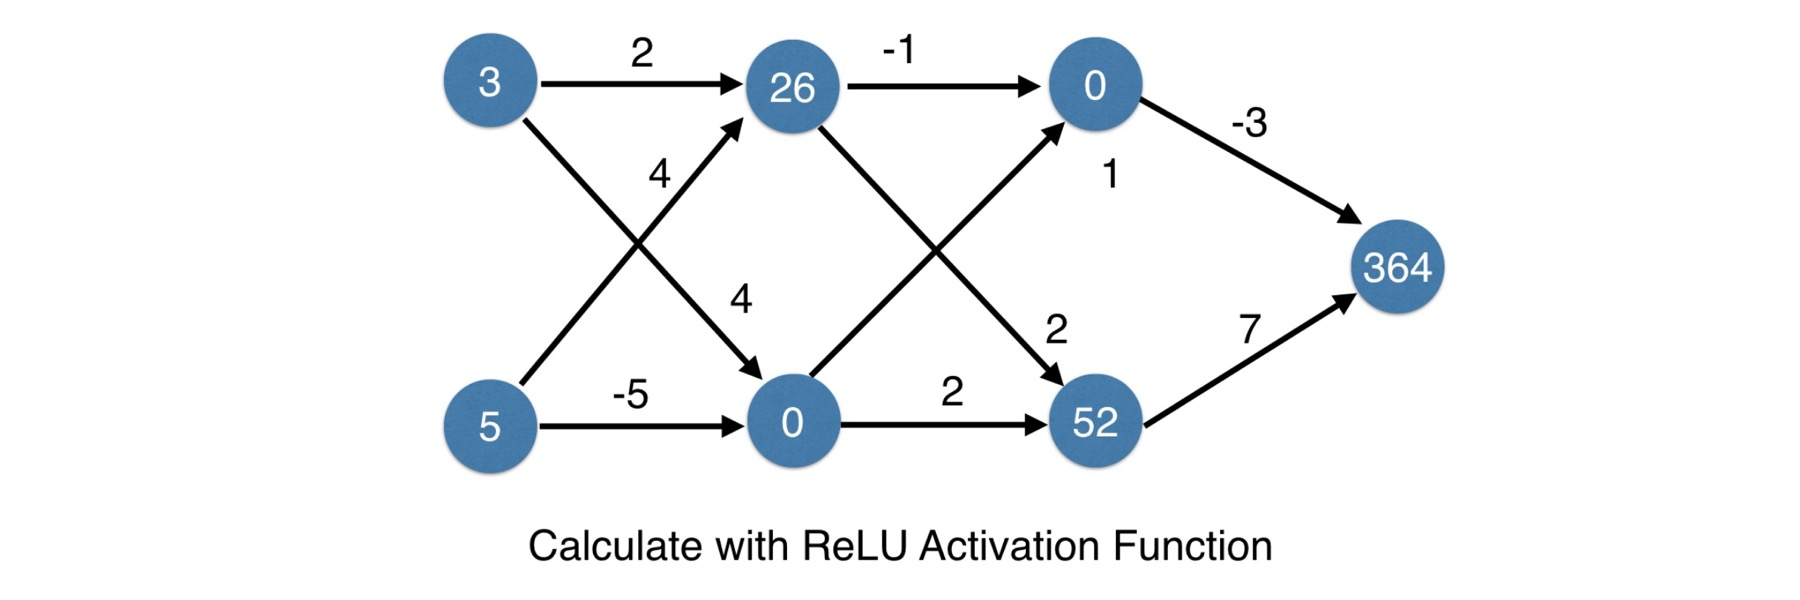
\includegraphics{../Figures/9. Multiple hidden layers.jpg}
\caption{Multiple hidden layers}
\end{figure}

    \hypertarget{note-2-representation-learning}{%
\subsection{\texorpdfstring{\texttt{{[}note-2{]}} Representation
learning}{{[}note-2{]} Representation learning}}\label{note-2-representation-learning}}

\begin{itemize}
\item
  Deep networks internally build representations of patterns in the
  data.
\item
  Partially replace the need for feature engineering.
\item
  Subsequent layers build increasingly sophisticated representations of
  raw data.
\end{itemize}

\begin{figure}
\centering
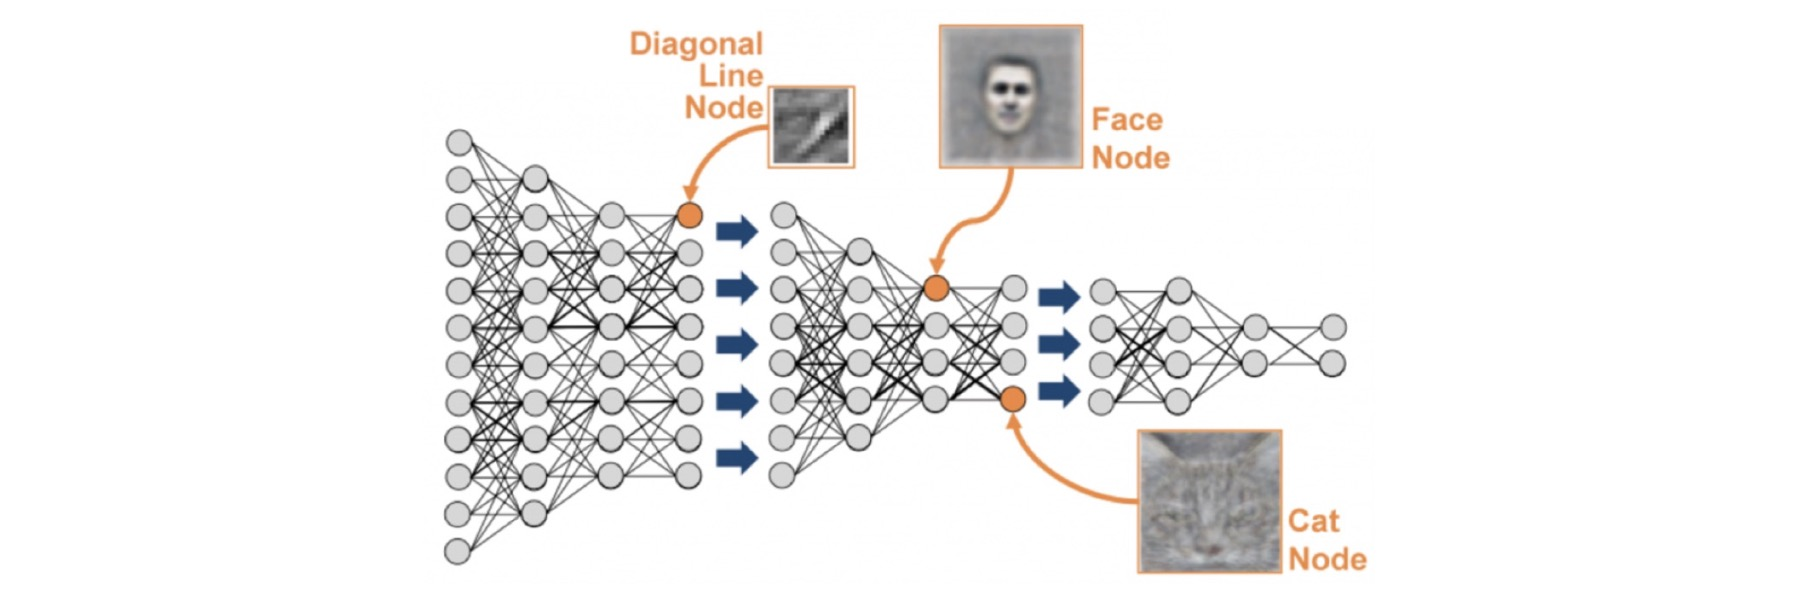
\includegraphics{../Figures/10. Representation learning.jpg}
\caption{Representation learning}
\end{figure}

    \hypertarget{note-3-deep-learning}{%
\subsection{\texorpdfstring{\texttt{{[}note-3{]}} Deep
learning}{{[}note-3{]} Deep learning}}\label{note-3-deep-learning}}

\begin{itemize}
\item
  The modeler doesn't need to specify the interactions.
\item
  When training the model, the neural network gets weights that find the
  relevant patterns to make better predictions.
\end{itemize}

    \hypertarget{quiz-1-forward-propagation-in-a-deeper-network}{%
\subsection{\texorpdfstring{\texttt{{[}quiz-1{]}} Forward propagation in
a deeper
network}{{[}quiz-1{]} Forward propagation in a deeper network}}\label{quiz-1-forward-propagation-in-a-deeper-network}}

\begin{itemize}
\item
  Ther is a model with two hidden layers. The values for an input data
  point are shown inside the input nodes. The weights are shown on the
  edges/lines. What prediction would this model make on this data point?
\item
  Assume the activation function at each node is the \emph{identity
  function}. That is, each node's output will be the same as its input.
  So the value of the bottom node in the first hidden layer is \(-1\),
  and not \(0\), as it would be if the ReLU activation function was
  used.

  \begin{figure}
  \centering
  
\includegraphics{../Figures/11. Forward propagation in a deeper network.png}
  \caption{Forward propagation in a deeper network}
  \end{figure}

  \(\boxtimes\) \(0\).

  \(\Box\) \(7\).

  \(\Box\) \(9\).
\end{itemize}

    \hypertarget{task-1-multi-layer-neural-networks}{%
\subsection{\texorpdfstring{\texttt{{[}task-1{]}} Multi-layer neural
networks}{{[}task-1{]} Multi-layer neural networks}}\label{task-1-multi-layer-neural-networks}}

\(\blacktriangleright\) \textbf{Task diagram}

\begin{figure}
\centering

\includegraphics{../Figures/12. Multi-layer neural networks.png}
\caption{Multi-layer neural networks}
\end{figure}

    \(\blacktriangleright\) \textbf{Package pre-loading}

    \begin{tcolorbox}[breakable, size=fbox, boxrule=1pt, pad at break*=1mm,colback=cellbackground, colframe=cellborder]
\prompt{In}{incolor}{12}{\boxspacing}
\begin{Verbatim}[commandchars=\\\{\}]
\PY{k+kn}{import} \PY{n+nn}{numpy} \PY{k}{as} \PY{n+nn}{np}
\end{Verbatim}
\end{tcolorbox}

    \(\blacktriangleright\) \textbf{Data pre-loading}

    \begin{tcolorbox}[breakable, size=fbox, boxrule=1pt, pad at break*=1mm,colback=cellbackground, colframe=cellborder]
\prompt{In}{incolor}{13}{\boxspacing}
\begin{Verbatim}[commandchars=\\\{\}]
\PY{n}{input\PYZus{}data} \PY{o}{=} \PY{n}{np}\PY{o}{.}\PY{n}{array}\PY{p}{(}\PY{p}{[}\PY{l+m+mi}{3}\PY{p}{,} \PY{l+m+mi}{5}\PY{p}{]}\PY{p}{)}

\PY{n}{weights} \PY{o}{=} \PY{p}{\PYZob{}}
    \PY{l+s+s1}{\PYZsq{}}\PY{l+s+s1}{node\PYZus{}0\PYZus{}0}\PY{l+s+s1}{\PYZsq{}}\PY{p}{:} \PY{n}{np}\PY{o}{.}\PY{n}{array}\PY{p}{(}\PY{p}{[}\PY{l+m+mi}{2}\PY{p}{,} \PY{l+m+mi}{4}\PY{p}{]}\PY{p}{)}\PY{p}{,}
    \PY{l+s+s1}{\PYZsq{}}\PY{l+s+s1}{node\PYZus{}0\PYZus{}1}\PY{l+s+s1}{\PYZsq{}}\PY{p}{:} \PY{n}{np}\PY{o}{.}\PY{n}{array}\PY{p}{(}\PY{p}{[}\PY{l+m+mi}{4}\PY{p}{,} \PY{o}{\PYZhy{}}\PY{l+m+mi}{5}\PY{p}{]}\PY{p}{)}\PY{p}{,}
    \PY{l+s+s1}{\PYZsq{}}\PY{l+s+s1}{node\PYZus{}1\PYZus{}0}\PY{l+s+s1}{\PYZsq{}}\PY{p}{:} \PY{n}{np}\PY{o}{.}\PY{n}{array}\PY{p}{(}\PY{p}{[}\PY{o}{\PYZhy{}}\PY{l+m+mi}{1}\PY{p}{,} \PY{l+m+mi}{2}\PY{p}{]}\PY{p}{)}\PY{p}{,}
    \PY{l+s+s1}{\PYZsq{}}\PY{l+s+s1}{node\PYZus{}1\PYZus{}1}\PY{l+s+s1}{\PYZsq{}}\PY{p}{:} \PY{n}{np}\PY{o}{.}\PY{n}{array}\PY{p}{(}\PY{p}{[}\PY{l+m+mi}{1}\PY{p}{,} \PY{l+m+mi}{2}\PY{p}{]}\PY{p}{)}\PY{p}{,}
    \PY{l+s+s1}{\PYZsq{}}\PY{l+s+s1}{output}\PY{l+s+s1}{\PYZsq{}}\PY{p}{:} \PY{n}{np}\PY{o}{.}\PY{n}{array}\PY{p}{(}\PY{p}{[}\PY{l+m+mi}{2}\PY{p}{,} \PY{l+m+mi}{7}\PY{p}{]}\PY{p}{)}
\PY{p}{\PYZcb{}}
\end{Verbatim}
\end{tcolorbox}

    \(\blacktriangleright\) \textbf{Code pre-loading}

    \begin{tcolorbox}[breakable, size=fbox, boxrule=1pt, pad at break*=1mm,colback=cellbackground, colframe=cellborder]
\prompt{In}{incolor}{14}{\boxspacing}
\begin{Verbatim}[commandchars=\\\{\}]
\PY{k}{def} \PY{n+nf}{relu}\PY{p}{(}\PY{n+nb}{input}\PY{p}{)}\PY{p}{:}
    \PY{n}{output} \PY{o}{=} \PY{n+nb}{max}\PY{p}{(}\PY{l+m+mi}{0}\PY{p}{,} \PY{n+nb}{input}\PY{p}{)}
    \PY{k}{return} \PY{p}{(}\PY{n}{output}\PY{p}{)}
\end{Verbatim}
\end{tcolorbox}

    \(\blacktriangleright\) \textbf{Task practice}

    \begin{tcolorbox}[breakable, size=fbox, boxrule=1pt, pad at break*=1mm,colback=cellbackground, colframe=cellborder]
\prompt{In}{incolor}{15}{\boxspacing}
\begin{Verbatim}[commandchars=\\\{\}]
\PY{k}{def} \PY{n+nf}{predict\PYZus{}with\PYZus{}network}\PY{p}{(}\PY{n}{input\PYZus{}data}\PY{p}{)}\PY{p}{:}
    \PY{c+c1}{\PYZsh{} Calculate node 0 in the first hidden layer}
    \PY{n}{node\PYZus{}0\PYZus{}0\PYZus{}input} \PY{o}{=} \PY{p}{(}\PY{n}{input\PYZus{}data} \PY{o}{*} \PY{n}{weights}\PY{p}{[}\PY{l+s+s1}{\PYZsq{}}\PY{l+s+s1}{node\PYZus{}0\PYZus{}0}\PY{l+s+s1}{\PYZsq{}}\PY{p}{]}\PY{p}{)}\PY{o}{.}\PY{n}{sum}\PY{p}{(}\PY{p}{)}
    \PY{n}{node\PYZus{}0\PYZus{}0\PYZus{}output} \PY{o}{=} \PY{n}{relu}\PY{p}{(}\PY{n}{node\PYZus{}0\PYZus{}0\PYZus{}input}\PY{p}{)}

    \PY{c+c1}{\PYZsh{} Calculate node 1 in the first hidden layer}
    \PY{n}{node\PYZus{}0\PYZus{}1\PYZus{}input} \PY{o}{=} \PY{p}{(}\PY{n}{input\PYZus{}data} \PY{o}{*} \PY{n}{weights}\PY{p}{[}\PY{l+s+s1}{\PYZsq{}}\PY{l+s+s1}{node\PYZus{}0\PYZus{}1}\PY{l+s+s1}{\PYZsq{}}\PY{p}{]}\PY{p}{)}\PY{o}{.}\PY{n}{sum}\PY{p}{(}\PY{p}{)}
    \PY{n}{node\PYZus{}0\PYZus{}1\PYZus{}output} \PY{o}{=} \PY{n}{relu}\PY{p}{(}\PY{n}{node\PYZus{}0\PYZus{}1\PYZus{}input}\PY{p}{)}

    \PY{c+c1}{\PYZsh{} Put node values into array: hidden\PYZus{}0\PYZus{}outputs}
    \PY{n}{hidden\PYZus{}0\PYZus{}outputs} \PY{o}{=} \PY{n}{np}\PY{o}{.}\PY{n}{array}\PY{p}{(}\PY{p}{[}\PY{n}{node\PYZus{}0\PYZus{}0\PYZus{}output}\PY{p}{,} \PY{n}{node\PYZus{}0\PYZus{}1\PYZus{}output}\PY{p}{]}\PY{p}{)}

    \PY{c+c1}{\PYZsh{} Calculate node 0 in the second hidden layer}
    \PY{n}{node\PYZus{}1\PYZus{}0\PYZus{}input} \PY{o}{=} \PY{p}{(}\PY{n}{hidden\PYZus{}0\PYZus{}outputs} \PY{o}{*} \PY{n}{weights}\PY{p}{[}\PY{l+s+s1}{\PYZsq{}}\PY{l+s+s1}{node\PYZus{}1\PYZus{}0}\PY{l+s+s1}{\PYZsq{}}\PY{p}{]}\PY{p}{)}\PY{o}{.}\PY{n}{sum}\PY{p}{(}\PY{p}{)}
    \PY{n}{node\PYZus{}1\PYZus{}0\PYZus{}output} \PY{o}{=} \PY{n}{relu}\PY{p}{(}\PY{n}{node\PYZus{}1\PYZus{}0\PYZus{}input}\PY{p}{)}

    \PY{c+c1}{\PYZsh{} Calculate node 1 in the second hidden layer}
    \PY{n}{node\PYZus{}1\PYZus{}1\PYZus{}input} \PY{o}{=} \PY{p}{(}\PY{n}{hidden\PYZus{}0\PYZus{}outputs} \PY{o}{*} \PY{n}{weights}\PY{p}{[}\PY{l+s+s1}{\PYZsq{}}\PY{l+s+s1}{node\PYZus{}1\PYZus{}1}\PY{l+s+s1}{\PYZsq{}}\PY{p}{]}\PY{p}{)}\PY{o}{.}\PY{n}{sum}\PY{p}{(}\PY{p}{)}
    \PY{n}{node\PYZus{}1\PYZus{}1\PYZus{}output} \PY{o}{=} \PY{n}{relu}\PY{p}{(}\PY{n}{node\PYZus{}1\PYZus{}1\PYZus{}input}\PY{p}{)}

    \PY{c+c1}{\PYZsh{} Put node values into array: hidden\PYZus{}1\PYZus{}outputs}
    \PY{n}{hidden\PYZus{}1\PYZus{}outputs} \PY{o}{=} \PY{n}{np}\PY{o}{.}\PY{n}{array}\PY{p}{(}\PY{p}{[}\PY{n}{node\PYZus{}1\PYZus{}0\PYZus{}output}\PY{p}{,} \PY{n}{node\PYZus{}1\PYZus{}1\PYZus{}output}\PY{p}{]}\PY{p}{)}

    \PY{c+c1}{\PYZsh{} Calculate model output: model\PYZus{}output}
    \PY{n}{model\PYZus{}output} \PY{o}{=} \PY{p}{(}\PY{n}{hidden\PYZus{}1\PYZus{}outputs} \PY{o}{*} \PY{n}{weights}\PY{p}{[}\PY{l+s+s1}{\PYZsq{}}\PY{l+s+s1}{output}\PY{l+s+s1}{\PYZsq{}}\PY{p}{]}\PY{p}{)}\PY{o}{.}\PY{n}{sum}\PY{p}{(}\PY{p}{)}

    \PY{c+c1}{\PYZsh{} Return model\PYZus{}output}
    \PY{k}{return} \PY{p}{(}\PY{n}{model\PYZus{}output}\PY{p}{)}


\PY{n}{output} \PY{o}{=} \PY{n}{predict\PYZus{}with\PYZus{}network}\PY{p}{(}\PY{n}{input\PYZus{}data}\PY{p}{)}
\PY{n+nb}{print}\PY{p}{(}\PY{n}{output}\PY{p}{)}
\end{Verbatim}
\end{tcolorbox}

    \begin{Verbatim}[commandchars=\\\{\}]
182
    \end{Verbatim}

    \hypertarget{quiz-2-representations-are-learned}{%
\subsection{\texorpdfstring{\texttt{{[}quiz-2{]}} Representations are
learned}{{[}quiz-2{]} Representations are learned}}\label{quiz-2-representations-are-learned}}

\begin{itemize}
\item
  How are the weights that determine the features/interactions in Neural
  Networks created?

  \(\Box\) A user chooses them when creating the model.

  \(\boxtimes\) The model training process sets them to optimize
  predictive accuracy.

  \(\Box\) The weights are random numbers.
\end{itemize}

    \hypertarget{quiz-3-levels-of-representation}{%
\subsection{\texorpdfstring{\texttt{{[}quiz-3{]}} Levels of
representation}{{[}quiz-3{]} Levels of representation}}\label{quiz-3-levels-of-representation}}

\begin{itemize}
\item
  Which layers of a model capture more complex or ``higher level''
  interactions?

  \(\Box\) The first layers capture the most complex interactions.

  \(\boxtimes\) The last layers capture the most complex interactions.

  \(\Box\) All layers capture interactions of similar complexity.
\end{itemize}

    \hypertarget{execution-environment}{%
\section{Execution environment}\label{execution-environment}}

    \begin{tcolorbox}[breakable, size=fbox, boxrule=1pt, pad at break*=1mm,colback=cellbackground, colframe=cellborder]
\prompt{In}{incolor}{16}{\boxspacing}
\begin{Verbatim}[commandchars=\\\{\}]
\PY{k+kn}{from} \PY{n+nn}{platform} \PY{k+kn}{import} \PY{n}{python\PYZus{}version}

\PY{n}{python\PYZus{}version} \PY{o}{=} \PY{p}{(}\PY{l+s+s1}{\PYZsq{}}\PY{l+s+s1}{python==}\PY{l+s+si}{\PYZob{}\PYZcb{}}\PY{l+s+s1}{\PYZsq{}}\PY{o}{.}\PY{n}{format}\PY{p}{(}\PY{n}{python\PYZus{}version}\PY{p}{(}\PY{p}{)}\PY{p}{)}\PY{p}{)}
\PY{n}{numpy\PYZus{}version} \PY{o}{=} \PY{p}{(}\PY{l+s+s1}{\PYZsq{}}\PY{l+s+s1}{numpy==}\PY{l+s+si}{\PYZob{}\PYZcb{}}\PY{l+s+s1}{\PYZsq{}}\PY{o}{.}\PY{n}{format}\PY{p}{(}\PY{n}{np}\PY{o}{.}\PY{n}{\PYZus{}\PYZus{}version\PYZus{}\PYZus{}}\PY{p}{)}\PY{p}{)}

\PY{n}{writepath} \PY{o}{=} \PY{l+s+s1}{\PYZsq{}}\PY{l+s+s1}{../../requirements.txt}\PY{l+s+s1}{\PYZsq{}}
\PY{n}{requirements} \PY{o}{=} \PY{p}{[}\PY{p}{]}
\PY{n}{packages} \PY{o}{=} \PY{p}{[}\PY{n}{numpy\PYZus{}version}\PY{p}{]}

\PY{k}{with} \PY{n+nb}{open}\PY{p}{(}\PY{n}{writepath}\PY{p}{,} \PY{l+s+s1}{\PYZsq{}}\PY{l+s+s1}{w+}\PY{l+s+s1}{\PYZsq{}}\PY{p}{)} \PY{k}{as} \PY{n}{file}\PY{p}{:}
    \PY{k}{for} \PY{n}{line} \PY{o+ow}{in} \PY{n}{file}\PY{p}{:}
        \PY{n}{requirements}\PY{o}{.}\PY{n}{append}\PY{p}{(}\PY{n}{line}\PY{o}{.}\PY{n}{strip}\PY{p}{(}\PY{l+s+s1}{\PYZsq{}}\PY{l+s+se}{\PYZbs{}n}\PY{l+s+s1}{\PYZsq{}}\PY{p}{)}\PY{p}{)}
    \PY{k}{for} \PY{n}{package} \PY{o+ow}{in} \PY{n}{packages}\PY{p}{:}
        \PY{k}{if} \PY{n}{package} \PY{o+ow}{not} \PY{o+ow}{in} \PY{n}{requirements}\PY{p}{:}
            \PY{n}{file}\PY{o}{.}\PY{n}{write}\PY{p}{(}\PY{n}{package} \PY{o}{+} \PY{l+s+s1}{\PYZsq{}}\PY{l+s+se}{\PYZbs{}n}\PY{l+s+s1}{\PYZsq{}}\PY{p}{)}

\PY{n}{max\PYZus{}characters} \PY{o}{=} \PY{n+nb}{len}\PY{p}{(}\PY{n}{python\PYZus{}version}\PY{p}{)}
\PY{k}{for} \PY{n}{package} \PY{o+ow}{in} \PY{n}{packages}\PY{p}{:}
    \PY{k}{if} \PY{n+nb}{max}\PY{p}{(}\PY{n}{max\PYZus{}characters}\PY{p}{,} \PY{n+nb}{len}\PY{p}{(}\PY{n}{package}\PY{p}{)}\PY{p}{)} \PY{o}{\PYZgt{}} \PY{n}{max\PYZus{}characters}\PY{p}{:}
        \PY{n}{max\PYZus{}characters} \PY{o}{=} \PY{n+nb}{max}\PY{p}{(}\PY{n}{max\PYZus{}characters}\PY{p}{,} \PY{n+nb}{len}\PY{p}{(}\PY{n}{package}\PY{p}{)}\PY{p}{)}

\PY{n+nb}{print}\PY{p}{(}\PY{l+s+s1}{\PYZsq{}}\PY{l+s+s1}{\PYZsh{}}\PY{l+s+s1}{\PYZsq{}} \PY{o}{*} \PY{p}{(}\PY{n}{max\PYZus{}characters} \PY{o}{+} \PY{l+m+mi}{8}\PY{p}{)}\PY{p}{)}
\PY{n+nb}{print}\PY{p}{(}\PY{l+s+s1}{\PYZsq{}}\PY{l+s+s1}{\PYZsh{}}\PY{l+s+s1}{\PYZsq{}} \PY{o}{*} \PY{l+m+mi}{2} \PY{o}{+} \PY{l+s+s1}{\PYZsq{}}\PY{l+s+s1}{ }\PY{l+s+s1}{\PYZsq{}} \PY{o}{*} \PY{p}{(}\PY{n}{max\PYZus{}characters} \PY{o}{+} \PY{l+m+mi}{4}\PY{p}{)} \PY{o}{+} \PY{l+s+s1}{\PYZsq{}}\PY{l+s+s1}{\PYZsh{}}\PY{l+s+s1}{\PYZsq{}} \PY{o}{*} \PY{l+m+mi}{2}\PY{p}{)}
\PY{n+nb}{print}\PY{p}{(}\PY{l+s+s1}{\PYZsq{}}\PY{l+s+s1}{\PYZsh{}}\PY{l+s+s1}{\PYZsq{}} \PY{o}{*} \PY{l+m+mi}{2} \PY{o}{+} \PY{l+s+s1}{\PYZsq{}}\PY{l+s+s1}{ }\PY{l+s+s1}{\PYZsq{}} \PY{o}{*} \PY{l+m+mi}{2} \PY{o}{+} \PY{n}{python\PYZus{}version} \PY{o}{+} \PY{l+s+s1}{\PYZsq{}}\PY{l+s+s1}{ }\PY{l+s+s1}{\PYZsq{}} \PY{o}{*}
      \PY{p}{(}\PY{n}{max\PYZus{}characters} \PY{o}{\PYZhy{}} \PY{n+nb}{len}\PY{p}{(}\PY{n}{python\PYZus{}version}\PY{p}{)} \PY{o}{+} \PY{l+m+mi}{2}\PY{p}{)} \PY{o}{+} \PY{l+s+s1}{\PYZsq{}}\PY{l+s+s1}{\PYZsh{}}\PY{l+s+s1}{\PYZsq{}} \PY{o}{*} \PY{l+m+mi}{2}\PY{p}{)}
\PY{n+nb}{print}\PY{p}{(}\PY{l+s+s1}{\PYZsq{}}\PY{l+s+s1}{\PYZsh{}}\PY{l+s+s1}{\PYZsq{}} \PY{o}{*} \PY{l+m+mi}{2} \PY{o}{+} \PY{l+s+s1}{\PYZsq{}}\PY{l+s+s1}{ }\PY{l+s+s1}{\PYZsq{}} \PY{o}{*} \PY{l+m+mi}{2} \PY{o}{+} \PY{n}{numpy\PYZus{}version} \PY{o}{+} \PY{l+s+s1}{\PYZsq{}}\PY{l+s+s1}{ }\PY{l+s+s1}{\PYZsq{}} \PY{o}{*}
      \PY{p}{(}\PY{n}{max\PYZus{}characters} \PY{o}{\PYZhy{}} \PY{n+nb}{len}\PY{p}{(}\PY{n}{numpy\PYZus{}version}\PY{p}{)} \PY{o}{+} \PY{l+m+mi}{2}\PY{p}{)} \PY{o}{+} \PY{l+s+s1}{\PYZsq{}}\PY{l+s+s1}{\PYZsh{}}\PY{l+s+s1}{\PYZsq{}} \PY{o}{*} \PY{l+m+mi}{2}\PY{p}{)}
\PY{n+nb}{print}\PY{p}{(}\PY{l+s+s1}{\PYZsq{}}\PY{l+s+s1}{\PYZsh{}}\PY{l+s+s1}{\PYZsq{}} \PY{o}{*} \PY{l+m+mi}{2} \PY{o}{+} \PY{l+s+s1}{\PYZsq{}}\PY{l+s+s1}{ }\PY{l+s+s1}{\PYZsq{}} \PY{o}{*} \PY{p}{(}\PY{n}{max\PYZus{}characters} \PY{o}{+} \PY{l+m+mi}{4}\PY{p}{)} \PY{o}{+} \PY{l+s+s1}{\PYZsq{}}\PY{l+s+s1}{\PYZsh{}}\PY{l+s+s1}{\PYZsq{}} \PY{o}{*} \PY{l+m+mi}{2}\PY{p}{)}
\PY{n+nb}{print}\PY{p}{(}\PY{l+s+s1}{\PYZsq{}}\PY{l+s+s1}{\PYZsh{}}\PY{l+s+s1}{\PYZsq{}} \PY{o}{*} \PY{p}{(}\PY{n}{max\PYZus{}characters} \PY{o}{+} \PY{l+m+mi}{8}\PY{p}{)}\PY{p}{)}
\end{Verbatim}
\end{tcolorbox}

    \begin{Verbatim}[commandchars=\\\{\}]
\#\#\#\#\#\#\#\#\#\#\#\#\#\#\#\#\#\#\#\#\#
\#\#                 \#\#
\#\#  python==3.7.9  \#\#
\#\#  numpy==1.19.5  \#\#
\#\#                 \#\#
\#\#\#\#\#\#\#\#\#\#\#\#\#\#\#\#\#\#\#\#\#
    \end{Verbatim}


    % Add a bibliography block to the postdoc
    
    
    
\end{document}
